% !TeX root = ../main.tex

\chapter{LAMMPS 的性能测试和分析}
通过前两章内容的描述,我们给出了在申威众核平台上针对 eFF 势函数在计算,访存,通信等多个方面的并行和优化方案。本章会继续在对具体算例的实验中对这些优化方案进行测试工作,实验会在神威·太湖之光上以优化策略的性能对比和在大规模节点上以扩展性的形式呈现,并且这里对每一步优化后的结果和误差都进行了正确性验证。本章分为三节,第一节给出在神威·太湖之光与通用平台上的硬件对比,以及在测试时使用到的不同类型和规模的算例介绍。第二节是针对不同优化策略和组合对于提升整体计算性能效果的测试,进而分析对于LAMMPS 计算下访存,通信等应用特征。最后通过扩展性测试给出优化策略在大规模节点下的性能展示。下面给出实验中用到的不同优化方案及其组合:

\section{实验配置及算例介绍}
\subsection{实验配置}
本文主要优化策略均在申威众核平台上进行,为对比不同平台间的性能差异,除在神威·太湖之光上进行测试之外,还进行了通用 X86 处理器平台上的性能分析对比实验,平台具体参数如下:

\begin{table}[]
     \centering
     \caption{SW26010 environment configuration}
       \renewcommand{\arraystretch}{1.5}
\begin{tabular}{lll}
\hline
       & SW26010 pro  & Intel Xeon CPU E5-2660 \\ \hline
主频(主核) & 1.45        & 2.2                    \\
主频(从核) & 1.45        & /                      \\
处理器核数 & 6MPEs/384CPEs & 12cores/24threads \\
内存     & 8           & 8                      \\
页表大小   & 8           & 4                      \\
网络 & 自研网络 & 系统总线 \\
并行环境 & Athread/MPI & MPI/OpenMP \\
指令集 & SW9 & AVX2 \\
编译器    & mpicc/sw5cc & mpicc                  \\ \hline
\end{tabular}
\end{table}

\subsection{实验算例}
针对 LAMMPS 中 eFF 势函数的计算,这里选取了冲击波诱导电离界面模拟。模拟体系中共包含三类粒子,氢原子核,锂原子核和电子。时间步选取为0.005fs,系综为 NVE,截断半径根据当前粒子类型动态决定,采用圆柱模型模拟,xy 方向为固定边界条件,z 方向采用周期性边界条件,初始温度为300,测试单位以每时间步耗时作为性能指标。

\begin{table}[]
  \centering
  \caption{实验算例配置及其参数}
  \renewcommand{\arraystretch}{1.5}
\begin{tabular}{lllll}
\hline
算例     & 粒子总数   & 类型    & 初始速度(kmd·$s^{-1}$) & 迭代步数  \\ \hline
RM\_S1 & 3000   & $Li/H_2$ & 22.50         & 5000  \\
RM\_S2 & 3000   & - & 45.00         & 20000 \\
RM\_M1 & 50000  & - & 45.00         & 5000  \\
RM\_M2 & 50000  & - & 22.50         & 20000 \\
RM\_L1 & 118000 & - & 22.50         & 5000  \\
RM\_L2 & 118000 & - & 45.50         & 20000 \\
RM\_L3 & 118000 & - & 22.50         & 20000 \\ \hline
\end{tabular}
\end{table}

eFF势算法主要进行常规环境与电离状态下的RM不稳定性研究,本文所涉及的实验内容将会包含如下算例。表5.2展示了不同算例下的模型分布。对于算例的选用,不同维度的模型参数对性能评估,加以不同权重的分析。

对于$Li/H_2$二维模型,激波压缩过程中,原子核与电子的扩散,随时间步形成电场,Li与H的粒子总量决定了整个模拟体系的规模。调整计算单元与粒子总量的比例,进行不同计算密度的映射,一方面可以进行优化手段与计算密度的对比,另一方面可以减少实验的自误差。

冲击激波自身提供电场与模拟空间的扩展动力,随着冲击速度的增加,电场内粒子的分离区域密度增加,且边界为刚体的情况下,模拟区域收缩,导致局部粒子密度的差异变化,从而产生划分区域及单核性能的波动。

对于体系模拟部分,在进行激波扩散前,需要对体系进行弛豫来保证局部是能最小化,使体系总能量保持在相对稳定的状态。本文选择了不同的运动时间步来区分不同阶段的运行比例,体现优化措施对于不同运行阶段的影响,以此评估在不同模拟时期的性能表现。

\subsection{正确性与性能评估}
RM不稳定性研究过程中,冲击波引发的高压缩强度,引起材料与微观尺度的动力学变化。本文设计模型以一侧刚体向内部释放冲击速度,引发激波对粒子的扰动,粒子性质与能量变化发生改变,经过再次平衡后,完成整个模拟过程的观察,在得出SW26010处理器模拟结果后,与天河平台的相同用例进行相同尺度的模拟比对,包括各时间步下粒子的坐标丶速度与受力情况统计等,完成基本模拟的正确性评估。

势函数算法性能测试作为本章实验内容的重点,在选择基准性能评估用例的同时,优化方案会同时采用多参数用例进行评估,一方面限制相对误差在合理阈值范围内,另一方面多用例输入能够对并行方案的峰值性能进行实际的期望统计,降低结果的随机性。在平台间的性能对比中,通过处理器结构间的差异,控制局部单一功能(cache,向量化),来观察特定优化策略与通用平台的性能差异。在整体扩展性测试阶段,这里选用相同系统状态,配置一致的用例为基础,进行eFF势算法研究上的强扩展性效率并行与弱扩展性效率并行测试,实现该模型在超大并行规模下的基准评估。

\section{峰值性能测试}
本文以模拟结果准确性与性能提升作为电子力场势(eFF)在LAMMPS上测试结果的指标,同时以不同维度与计算规模评估整个实验部分。多维的粒子数据类型与规模提升了模拟结果的准确性,复杂模型及边界条件的使用降低了评估误差。本章的测试针对eFF势函数计算,分别运行基准对照组串行版本,并行版本与不同优化措施下的优化版本,并根据其结果设置相对应的误差阈值,来保证结果的正确性。

\subsection{串行及粗粒度并行}
\subsubsection{主核串行}
图5.1表示LAMMPS在主核版本的性能表现,从不同算例的表现可以看出,主核版本的计算性能与计算规模基本呈正相关,计算规模与计算单元同比例增加,主核扩展性保持稳定。对于SW26010处理器核组使用,仅利用主核完成全部的计算以及相关的任务加载与调度,过程中从核核组来进行任何计算的参与,可以看出,此时整体性能并不理想,单个时间步耗时基本不可接受。此时主要的性能瓶颈在于整体计算负载在从核核组上的分配与平衡。
 \begin{figure}[h]
  \centering
  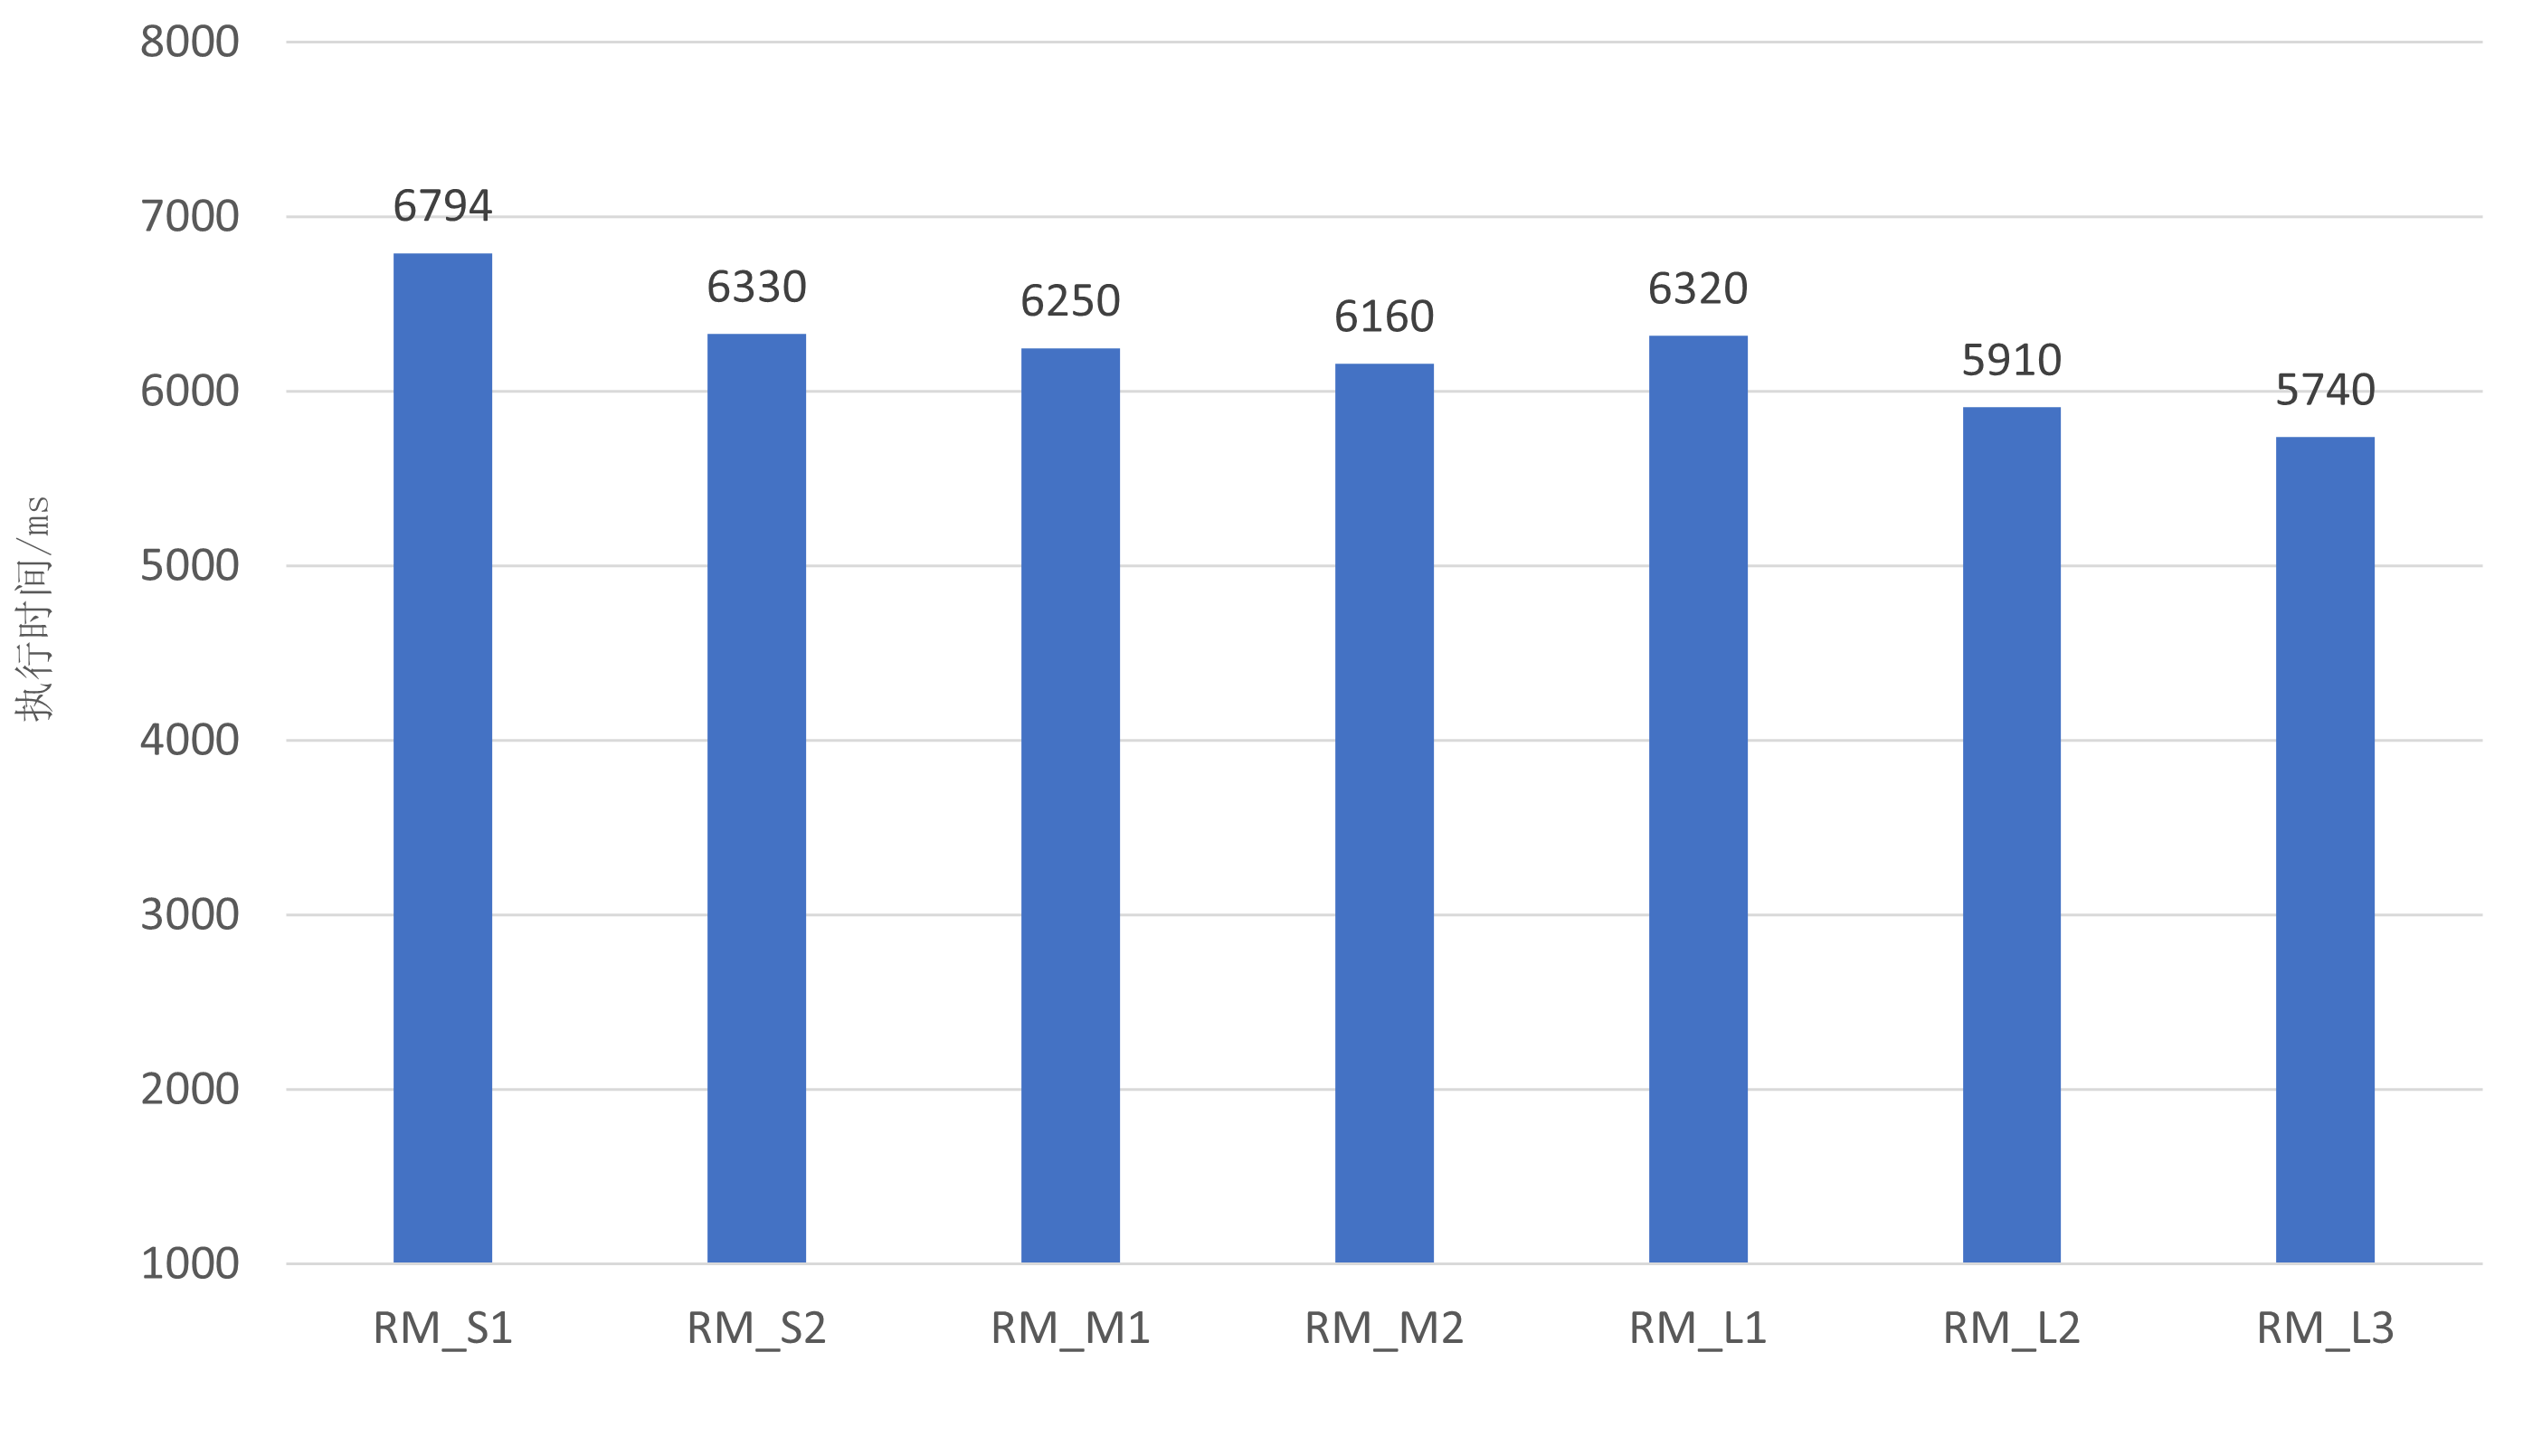
\includegraphics[width=0.8\textwidth]{e1.png}
  \caption{串行版本算例性能}
\end{figure}

\subsubsection{粗粒度并行}
图5.2展示了eFF势算法在基本并行版本下的性能表现,此时相对比主核版本,仅将算法中的热点计算部分分配到从核核组上进行协同计算,主核作为非耗时计算的承载者,与从核的调度者存在。相对于主核版本,从核核组的调用提高了计算负载的性能,用例平均性能提升了14.90倍。而在从核访存中,使用gld/gst直接访问主存地址进行低效数据交换,64个从核协同计算由于未进行相关优化操作,粒子数据依赖对结果的受力产生制约。对于计算流程中粒子局部性特征以及未对从核LDM充分利用,成为了当前方案面临的主要瓶颈。\\ \\ \\ \\ \\ \\
 \begin{figure}[h]
  \centering
  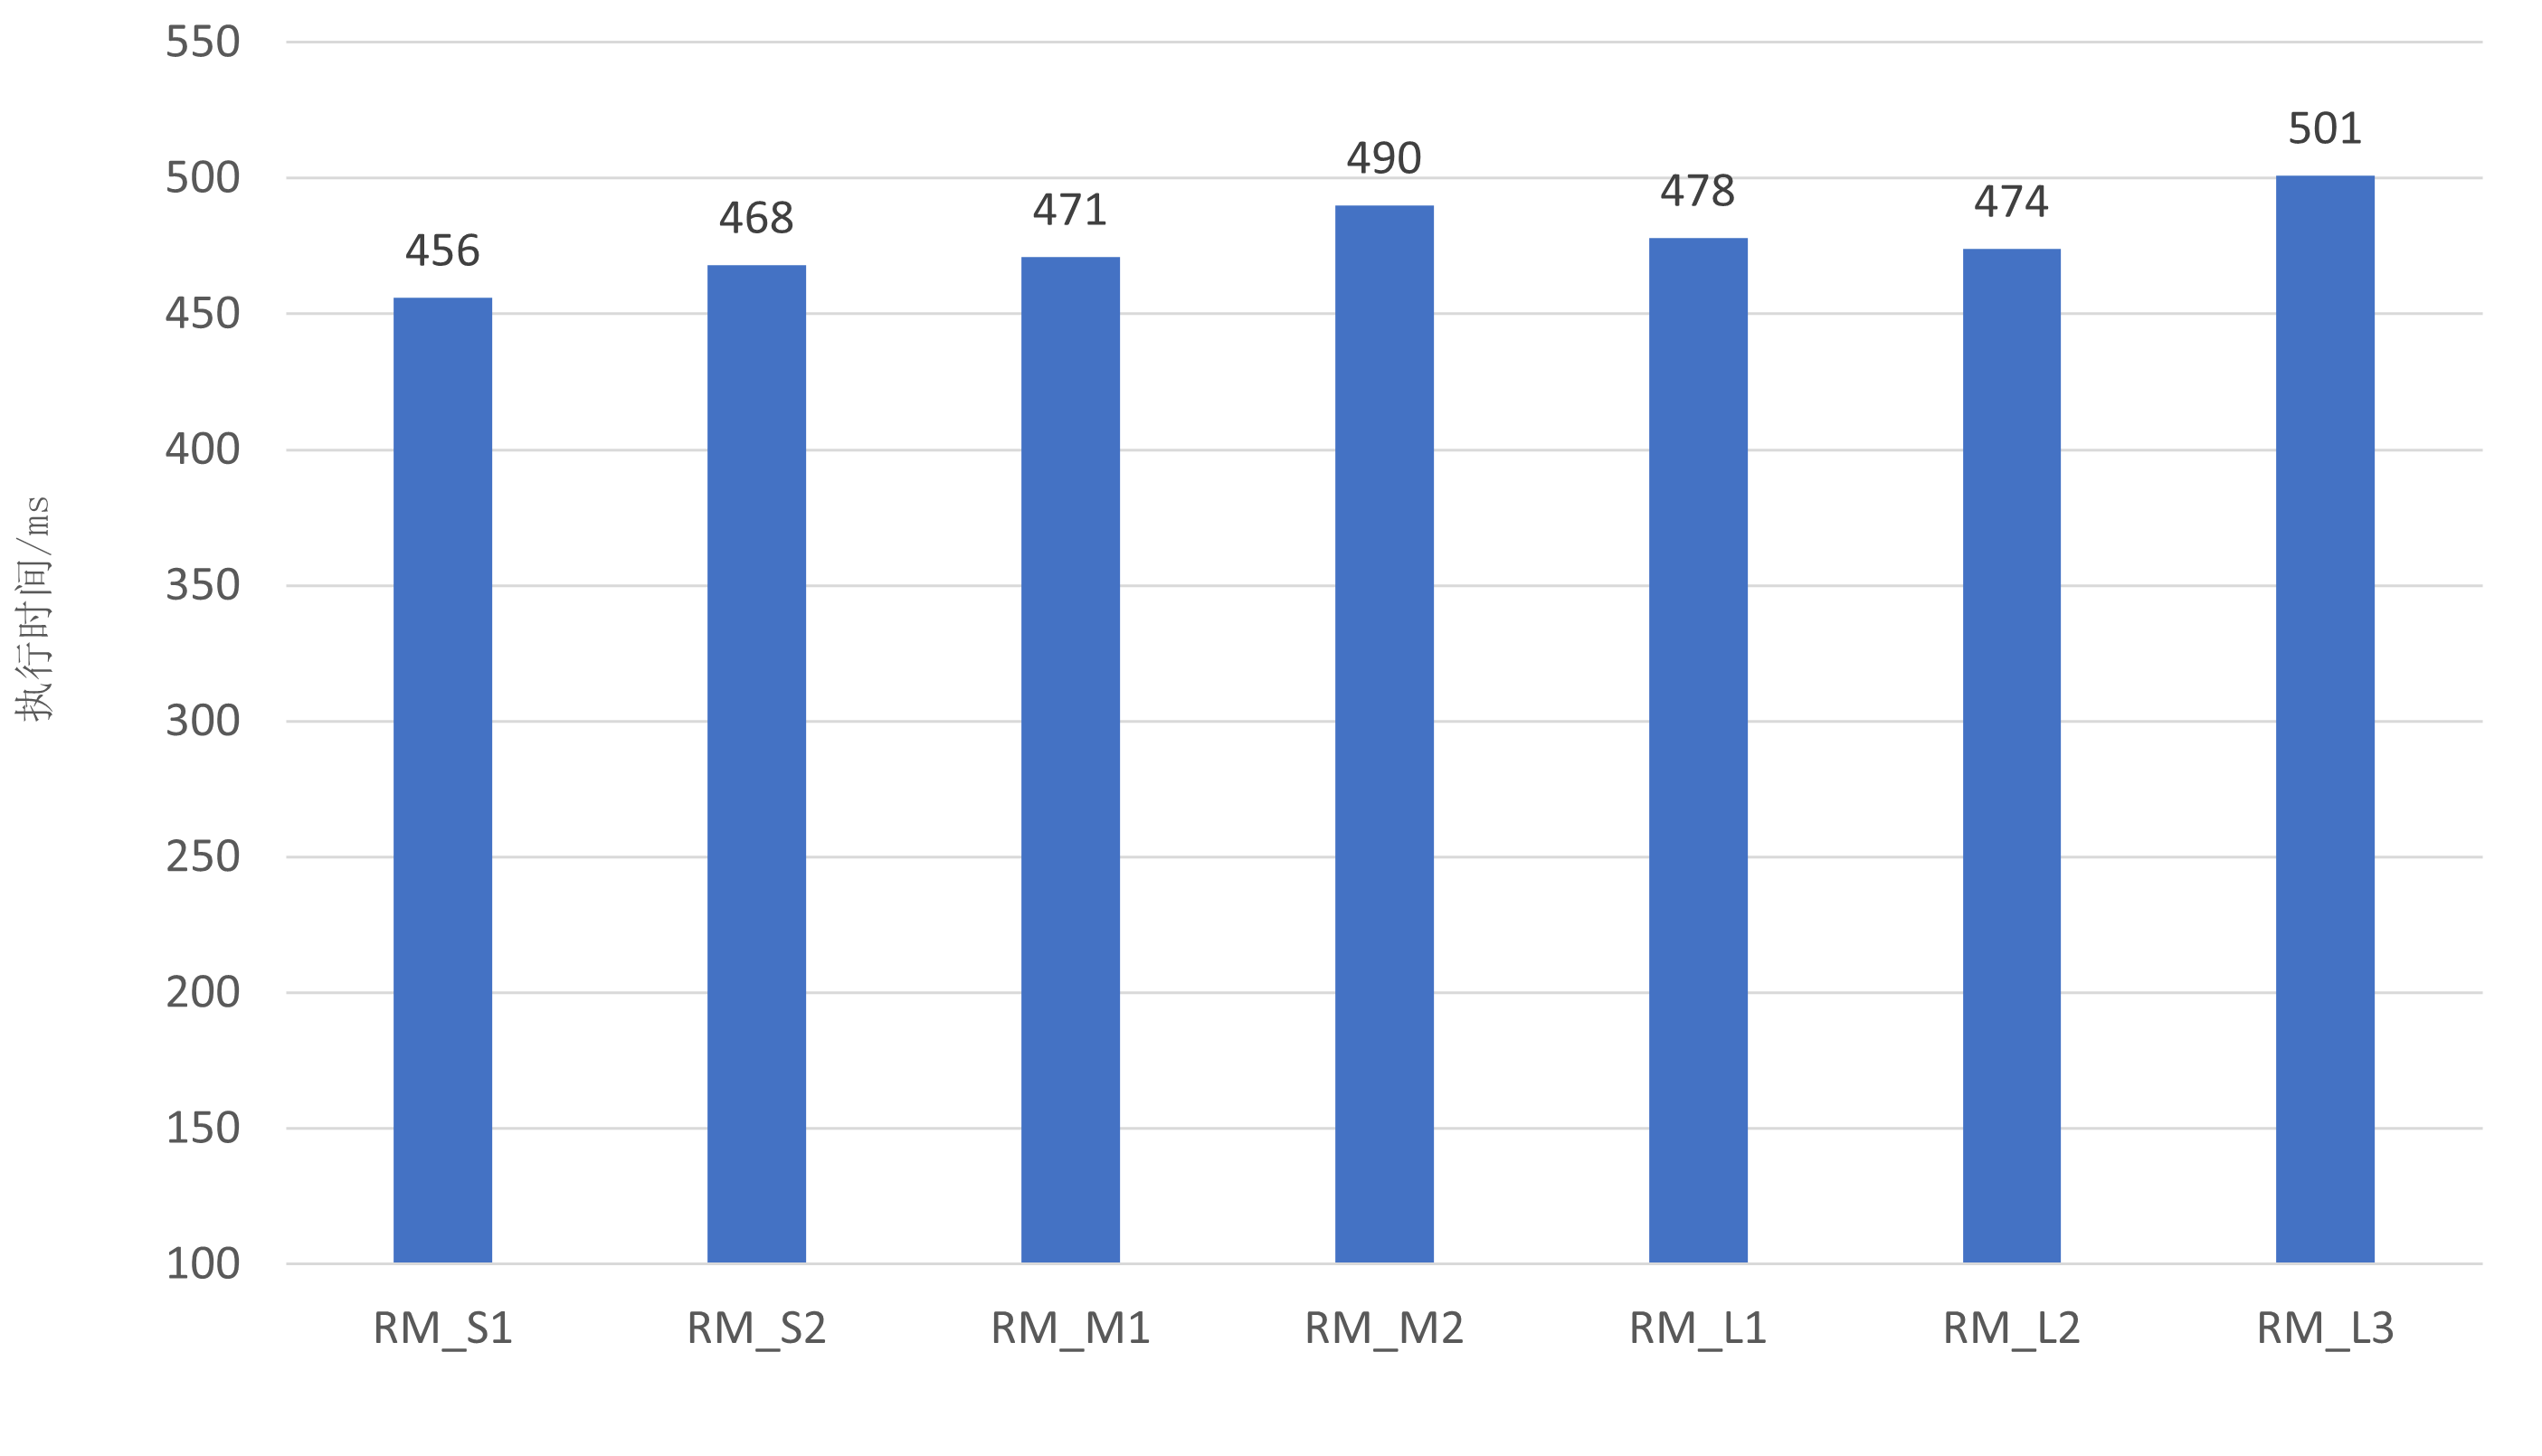
\includegraphics[width=0.8\textwidth]{e2.png}
  \caption{粗粒度并行算例性能}
\end{figure}

\subsection{细粒度并行及通用优化}
\subsubsection{单端并行}
图5.3展示了eFF势算法在采用单端并行算法后的性能表现。此时在将计算热点加载到从核核组的基础上,将粒子对间计算拆分为两次进行,降低粒子数据写依赖,拆分两层粒子循环,平衡访存与计算负载,用例平均性能提升了1.87倍左右。在充分利用从核核组计算资源后,计算量的上升,带来了访存,通信带宽与计算三方面的压力。
 \begin{figure}[h]
  \centering
  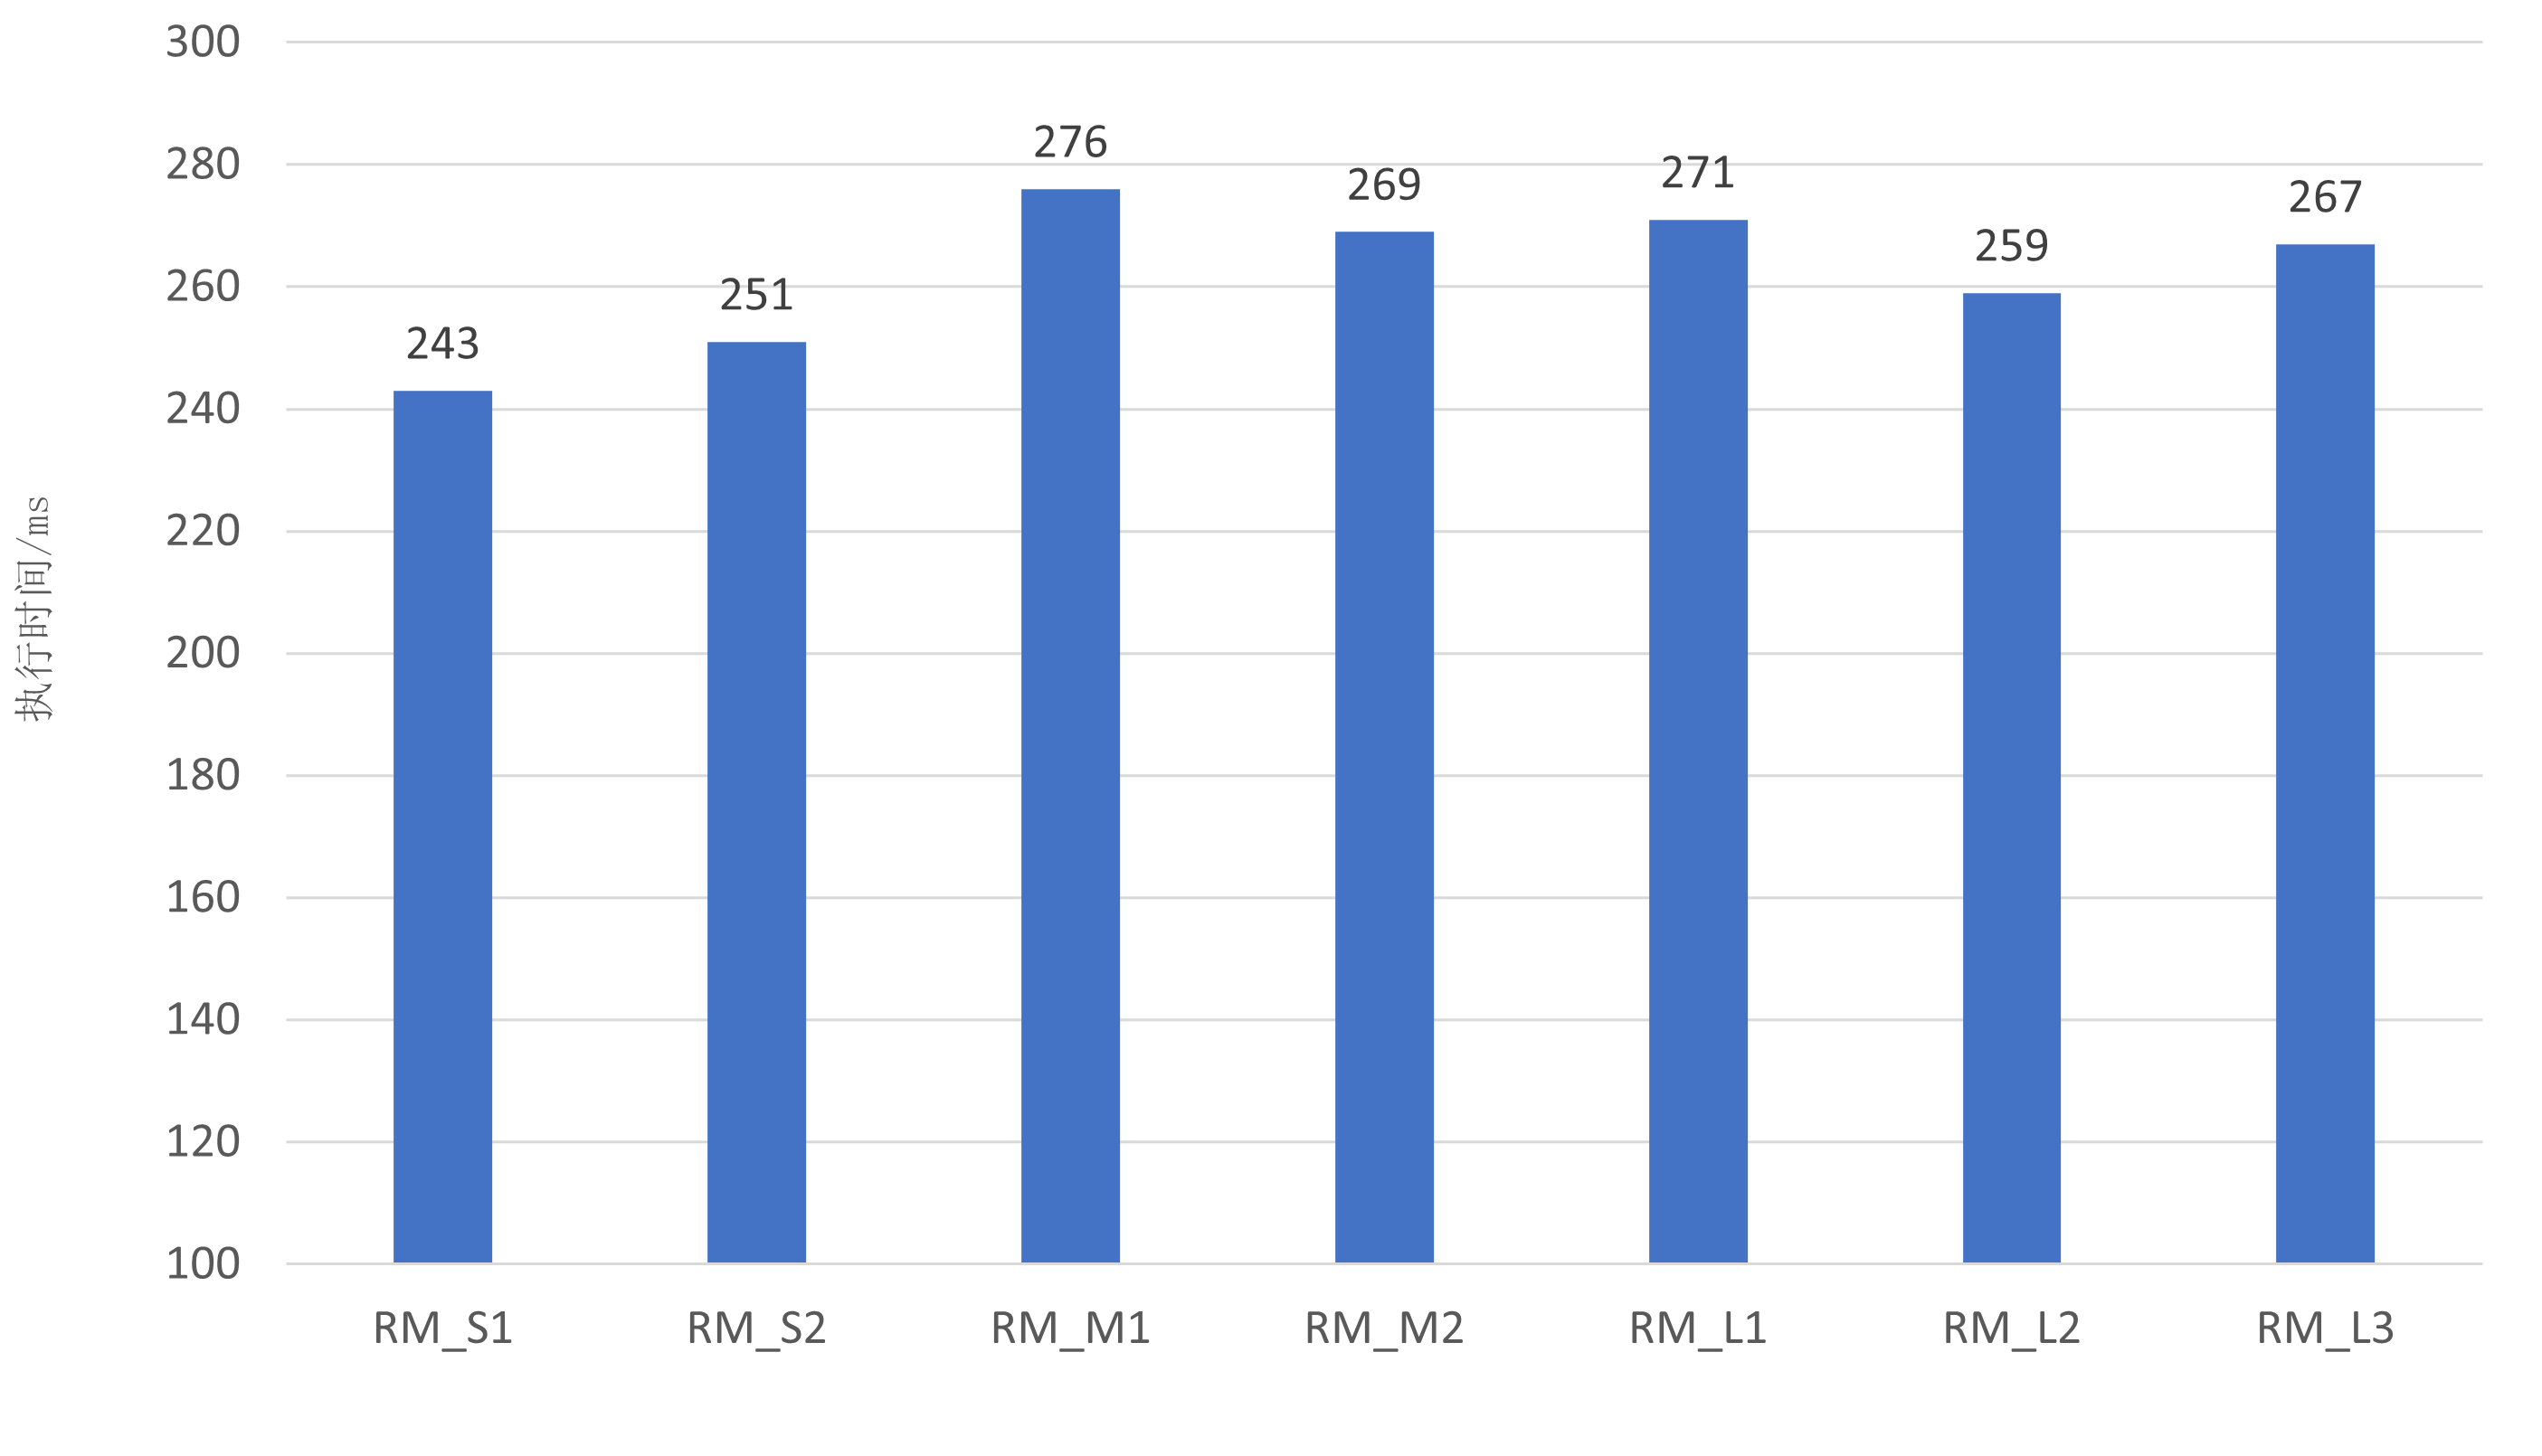
\includegraphics[width=0.8\textwidth]{e3.png}
  \caption{单端并行算例性能}
\end{figure}

\subsubsection{访存优化}
图5.4展示了eFF势算法在采用从核访存优化之后的性能表现。DMA访存接口调用对数据块大小较为敏感,并在读写初期需要初始化操作,在通过分析后充分利用通信带宽,DMA能够在连续访存时提高读写性能。预取方式的调用,对于粒子数据初期访问的性能波动产生了较优的效果,适用于粒子密度大的模拟体系。采用DMA访存与预取暂存策略获得了1.5倍的性能提升。
 \begin{figure}[h]
  \centering
  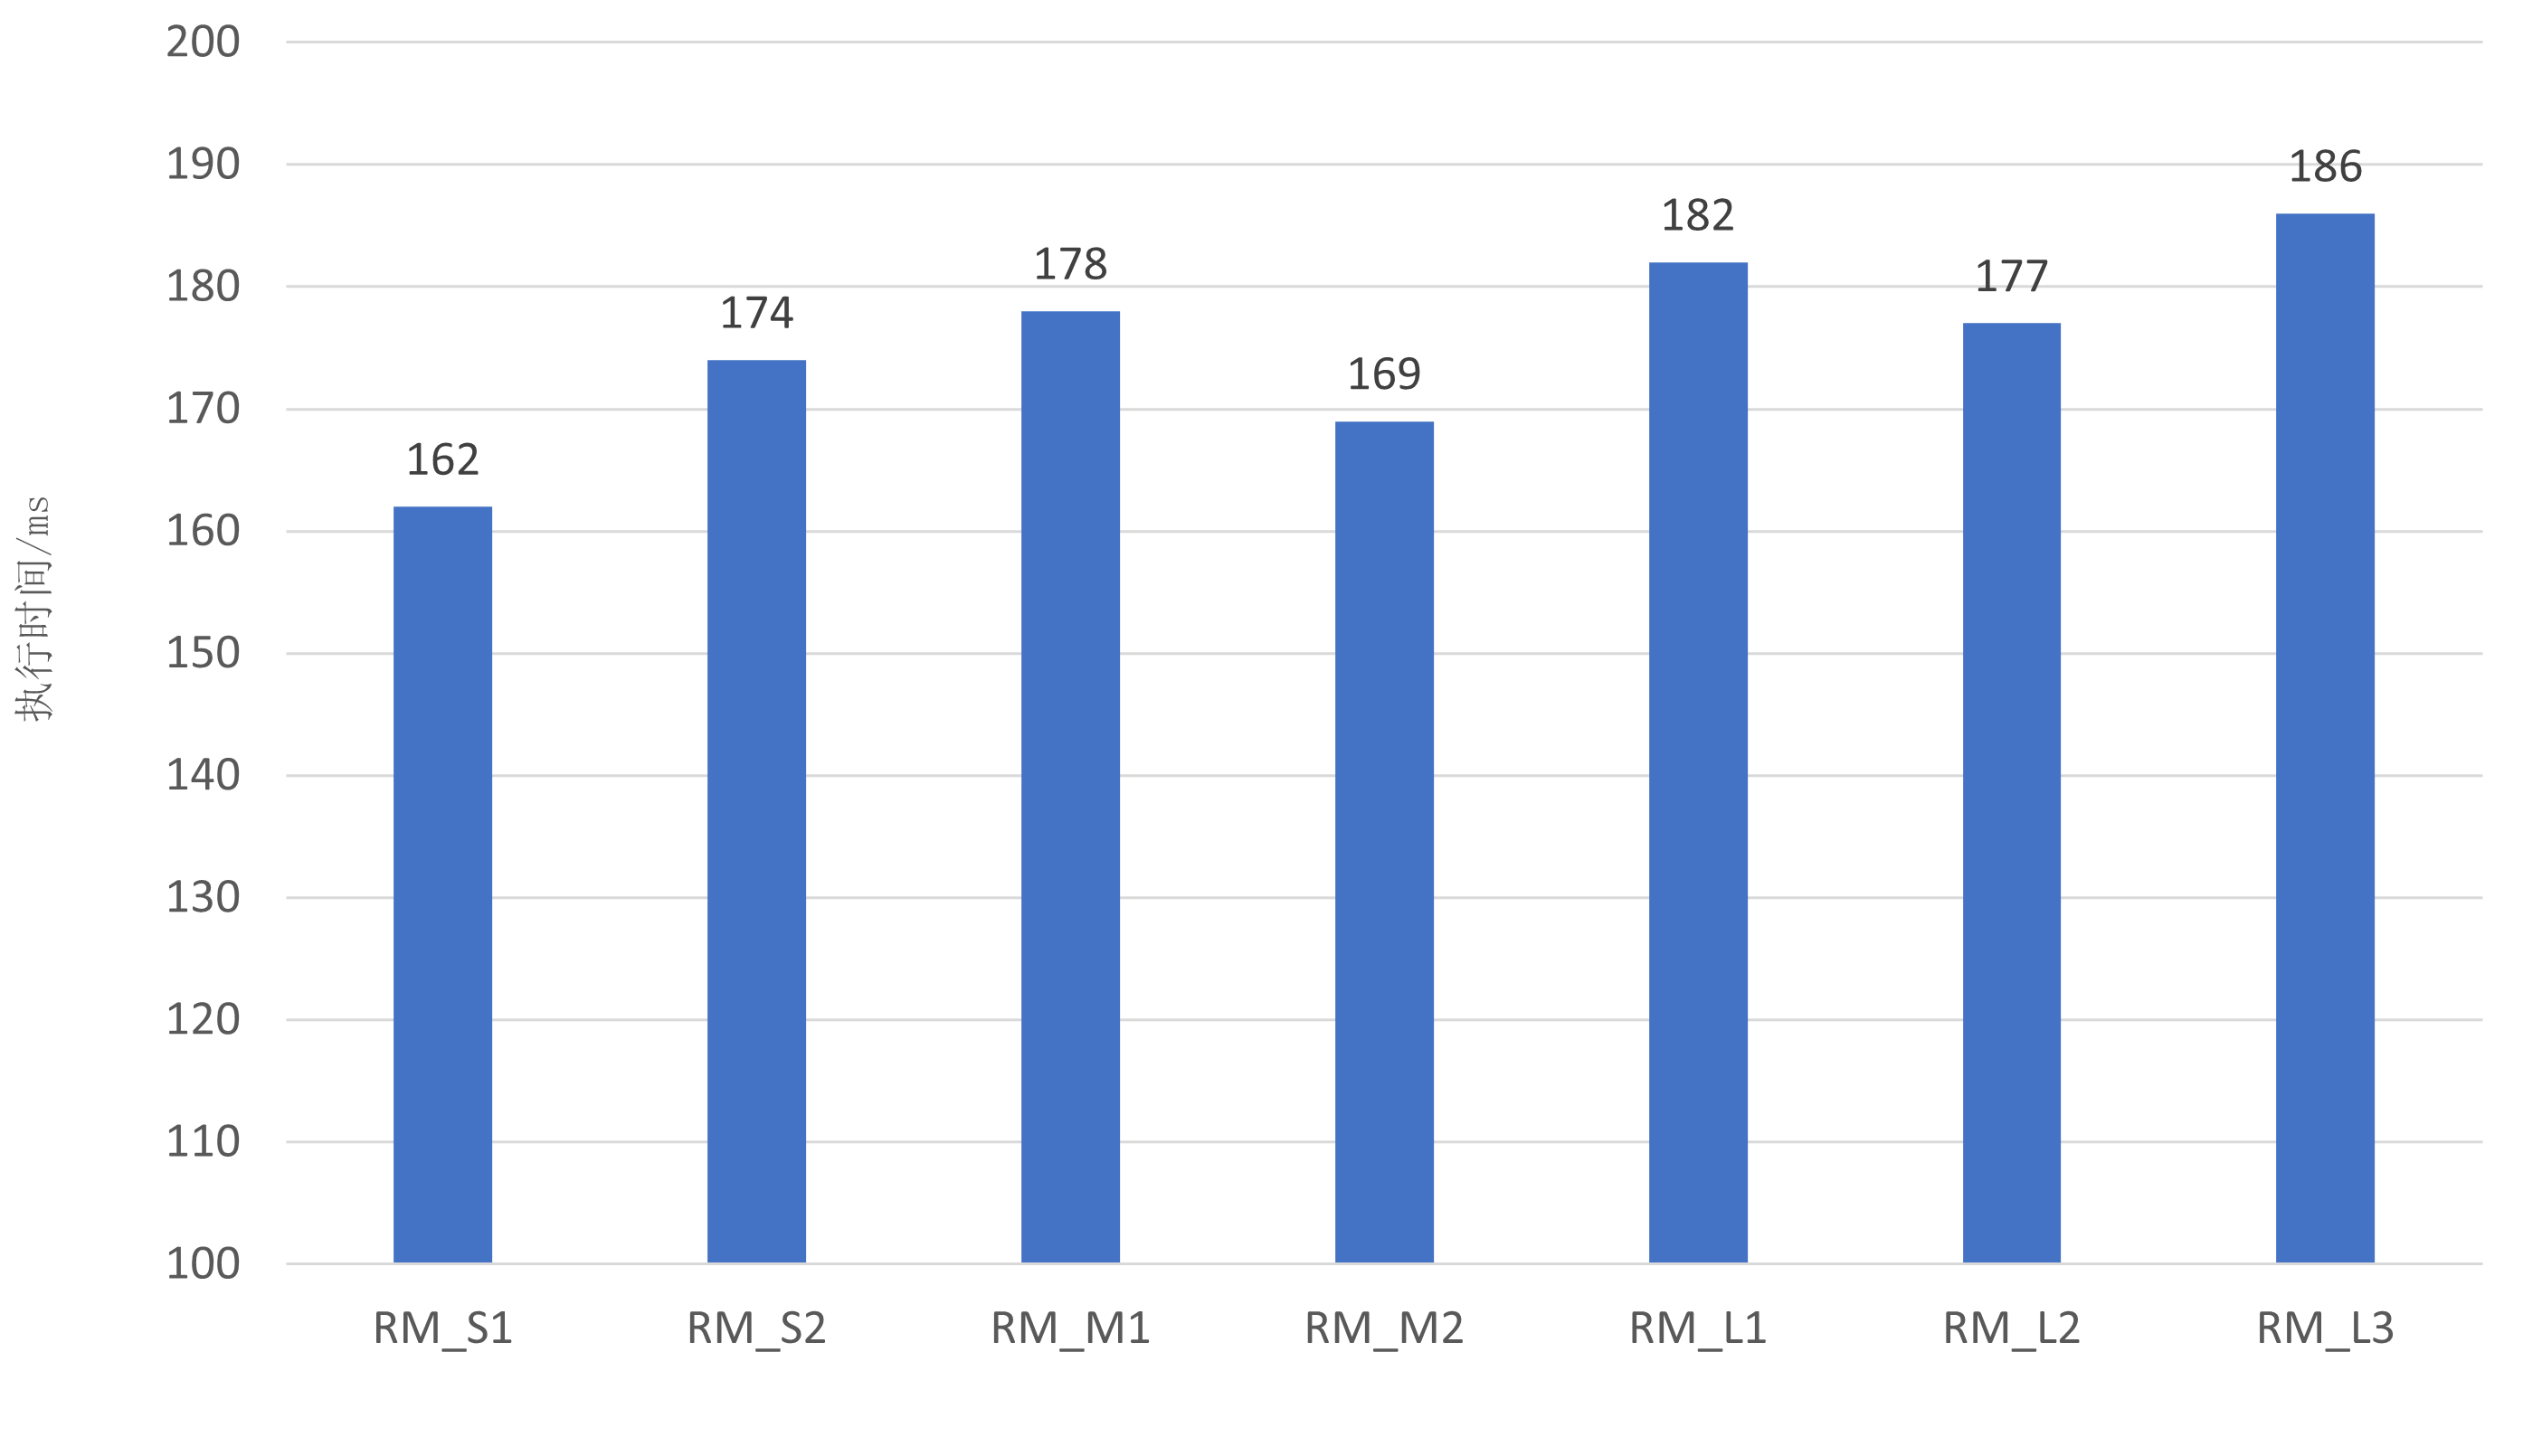
\includegraphics[width=0.8\textwidth]{e4.png}
  \caption{访存优化算例性能}
\end{figure}

\subsubsection{软件cache优化}
图5.5展示了eFF势算法在采用软件cache优化策略后的性能表现。对粒子数据局部性的捕捉,以及从核LDM局存的设计,提升了粒子数据重用的频率。在减少冗余访存的同时降低了带宽压力,通过软件cache的优化措施获得了约1.52倍的性能提升。直接映射的结构设计避免了软件指令带来过高的复杂度,对粒子数据的打包拆分保证在cache页内可以对其访问数据结构。在针对访存进行多角度优化后,计算占比在整个势函数计算中逐步提高,成为了影响性能提升的瓶颈。
 \begin{figure}[h]
  \centering
  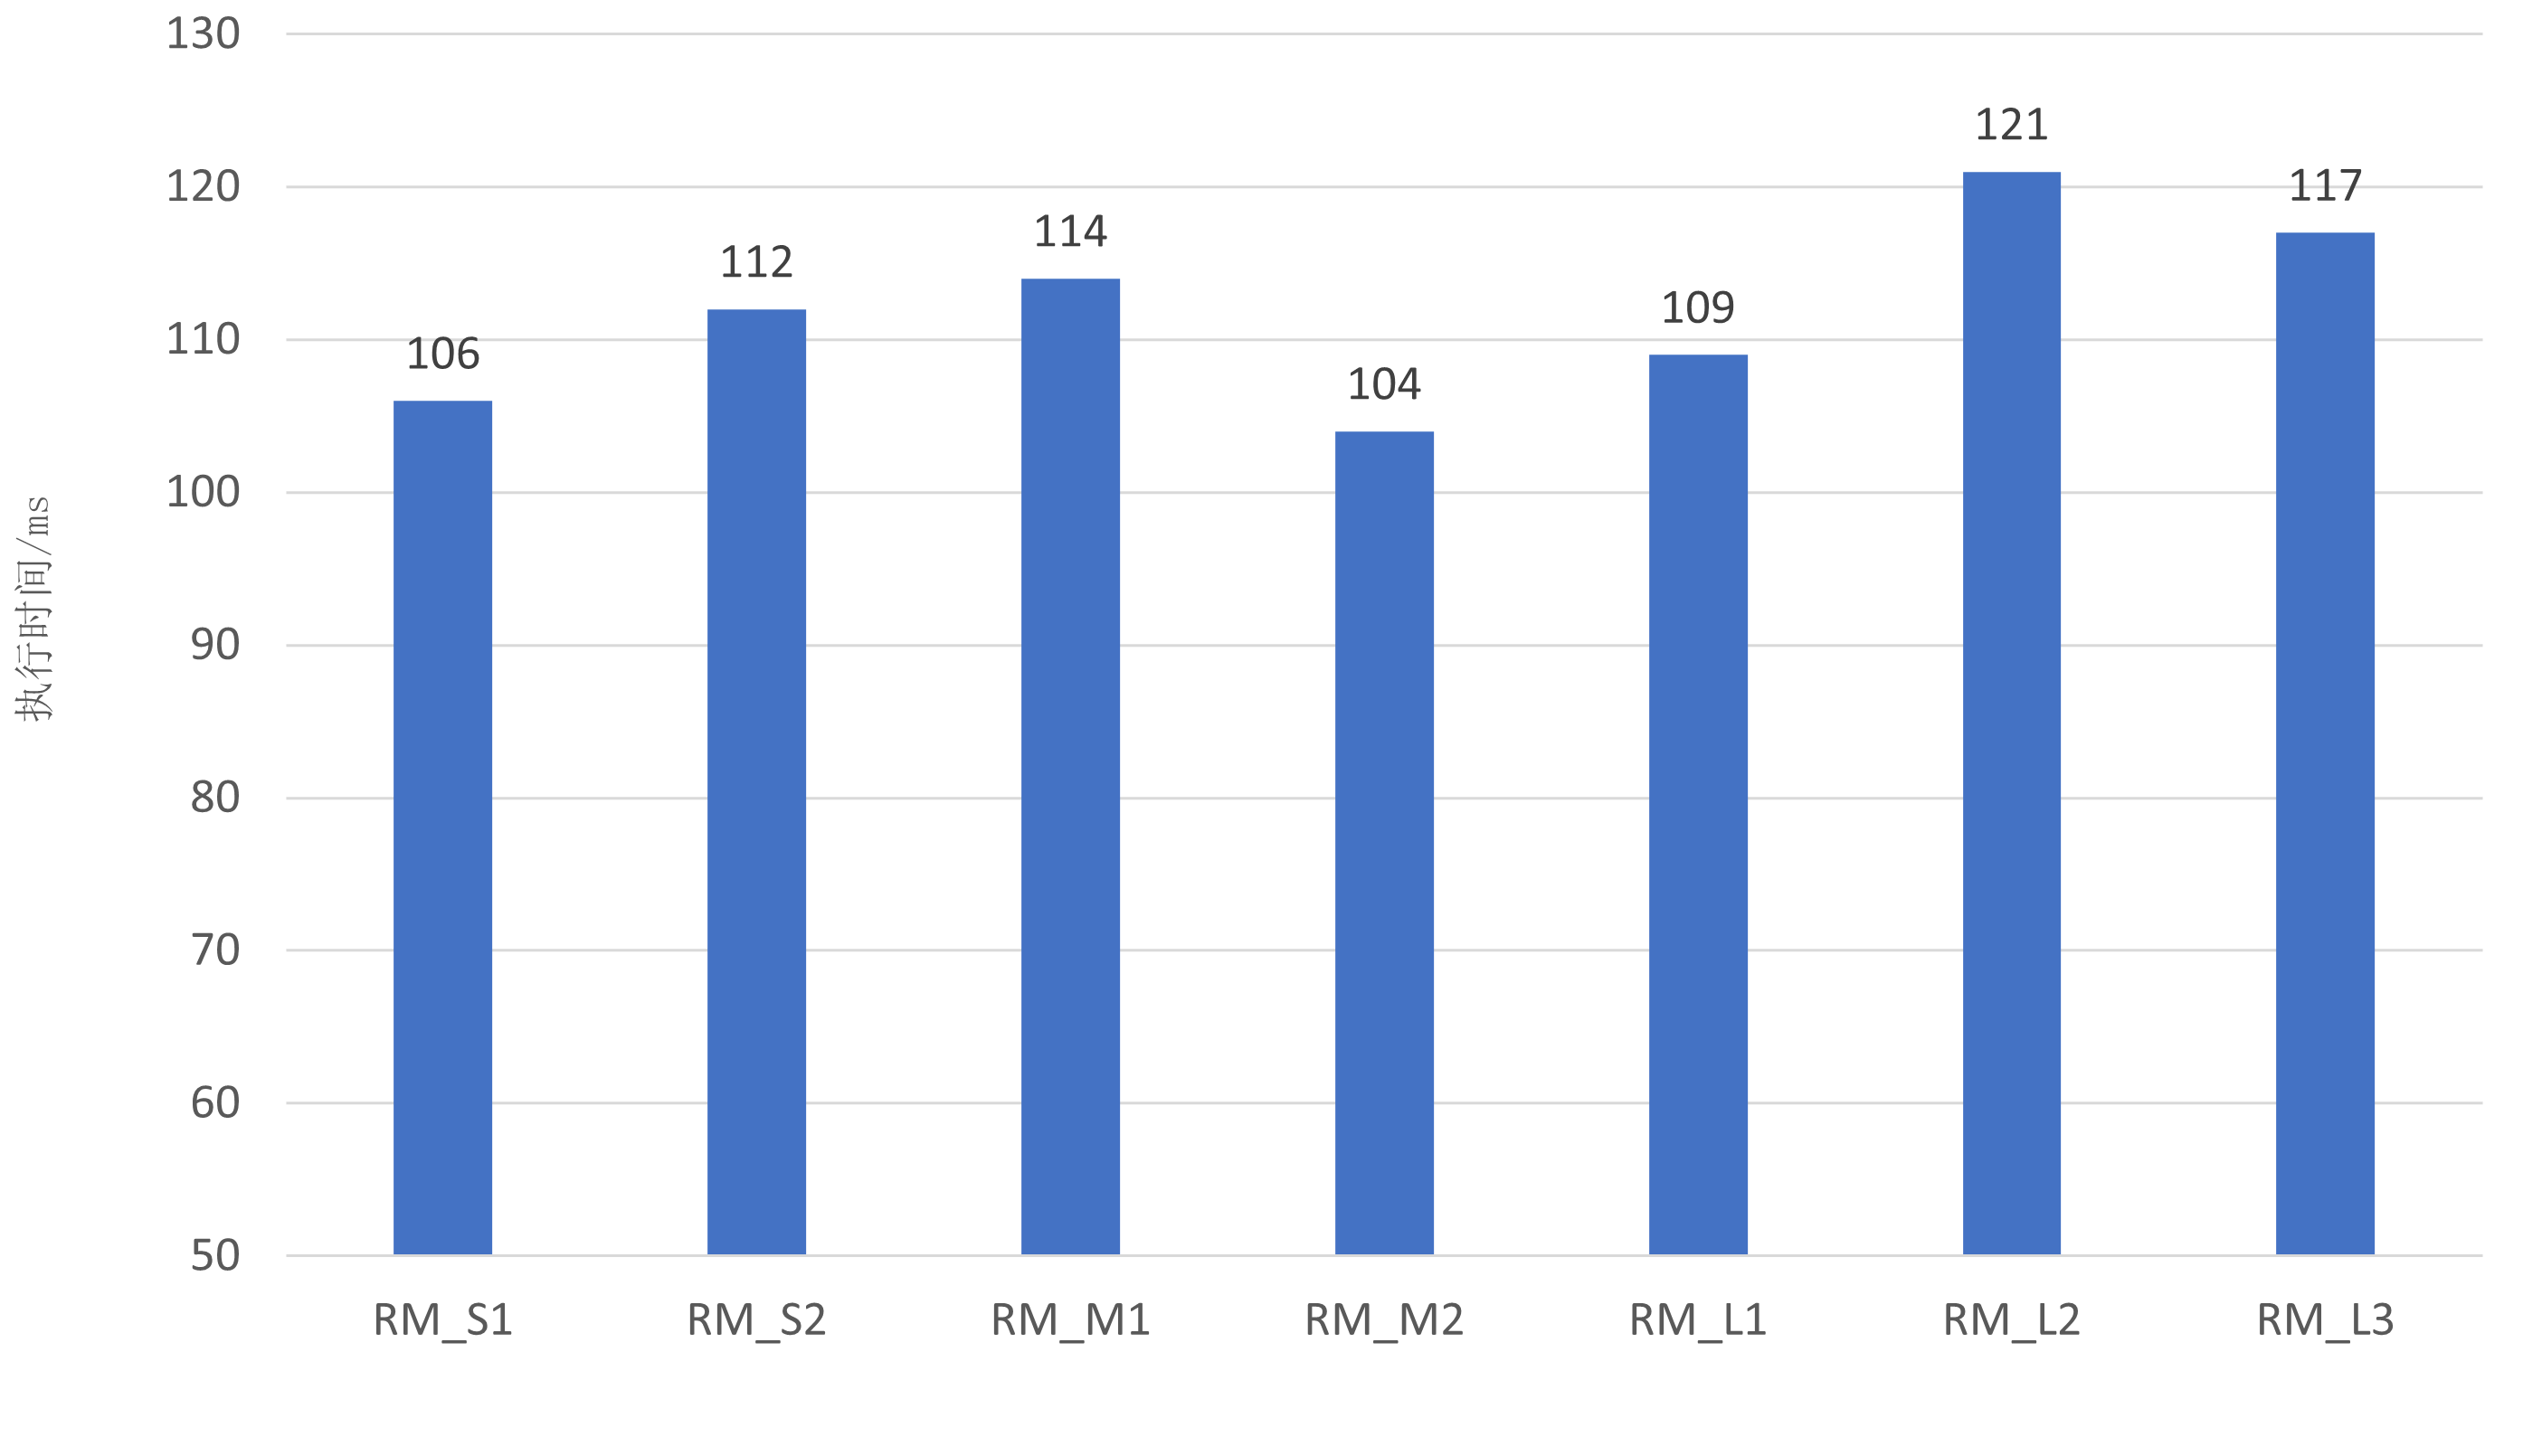
\includegraphics[width=0.8\textwidth]{e5.png}
  \caption{软件cache算例性能}
\end{figure}

\subsubsection{向量化}
图5.6展示了eFF势算法在采用向量化计算优化策略的性能表现,访存优化及并行策略的更新加大了计算在模拟流程中的占比。这里利用256位浮点向量化指令,单次打包4组粒子,使用向量混洗与向量计算,分配源向量及目标向量,向量化操作获得了约1.43倍的性能提升。此外解决了向量化在截断半径判断与粒子类型选择上的分支阻塞问题。
 \begin{figure}[h]
  \centering
  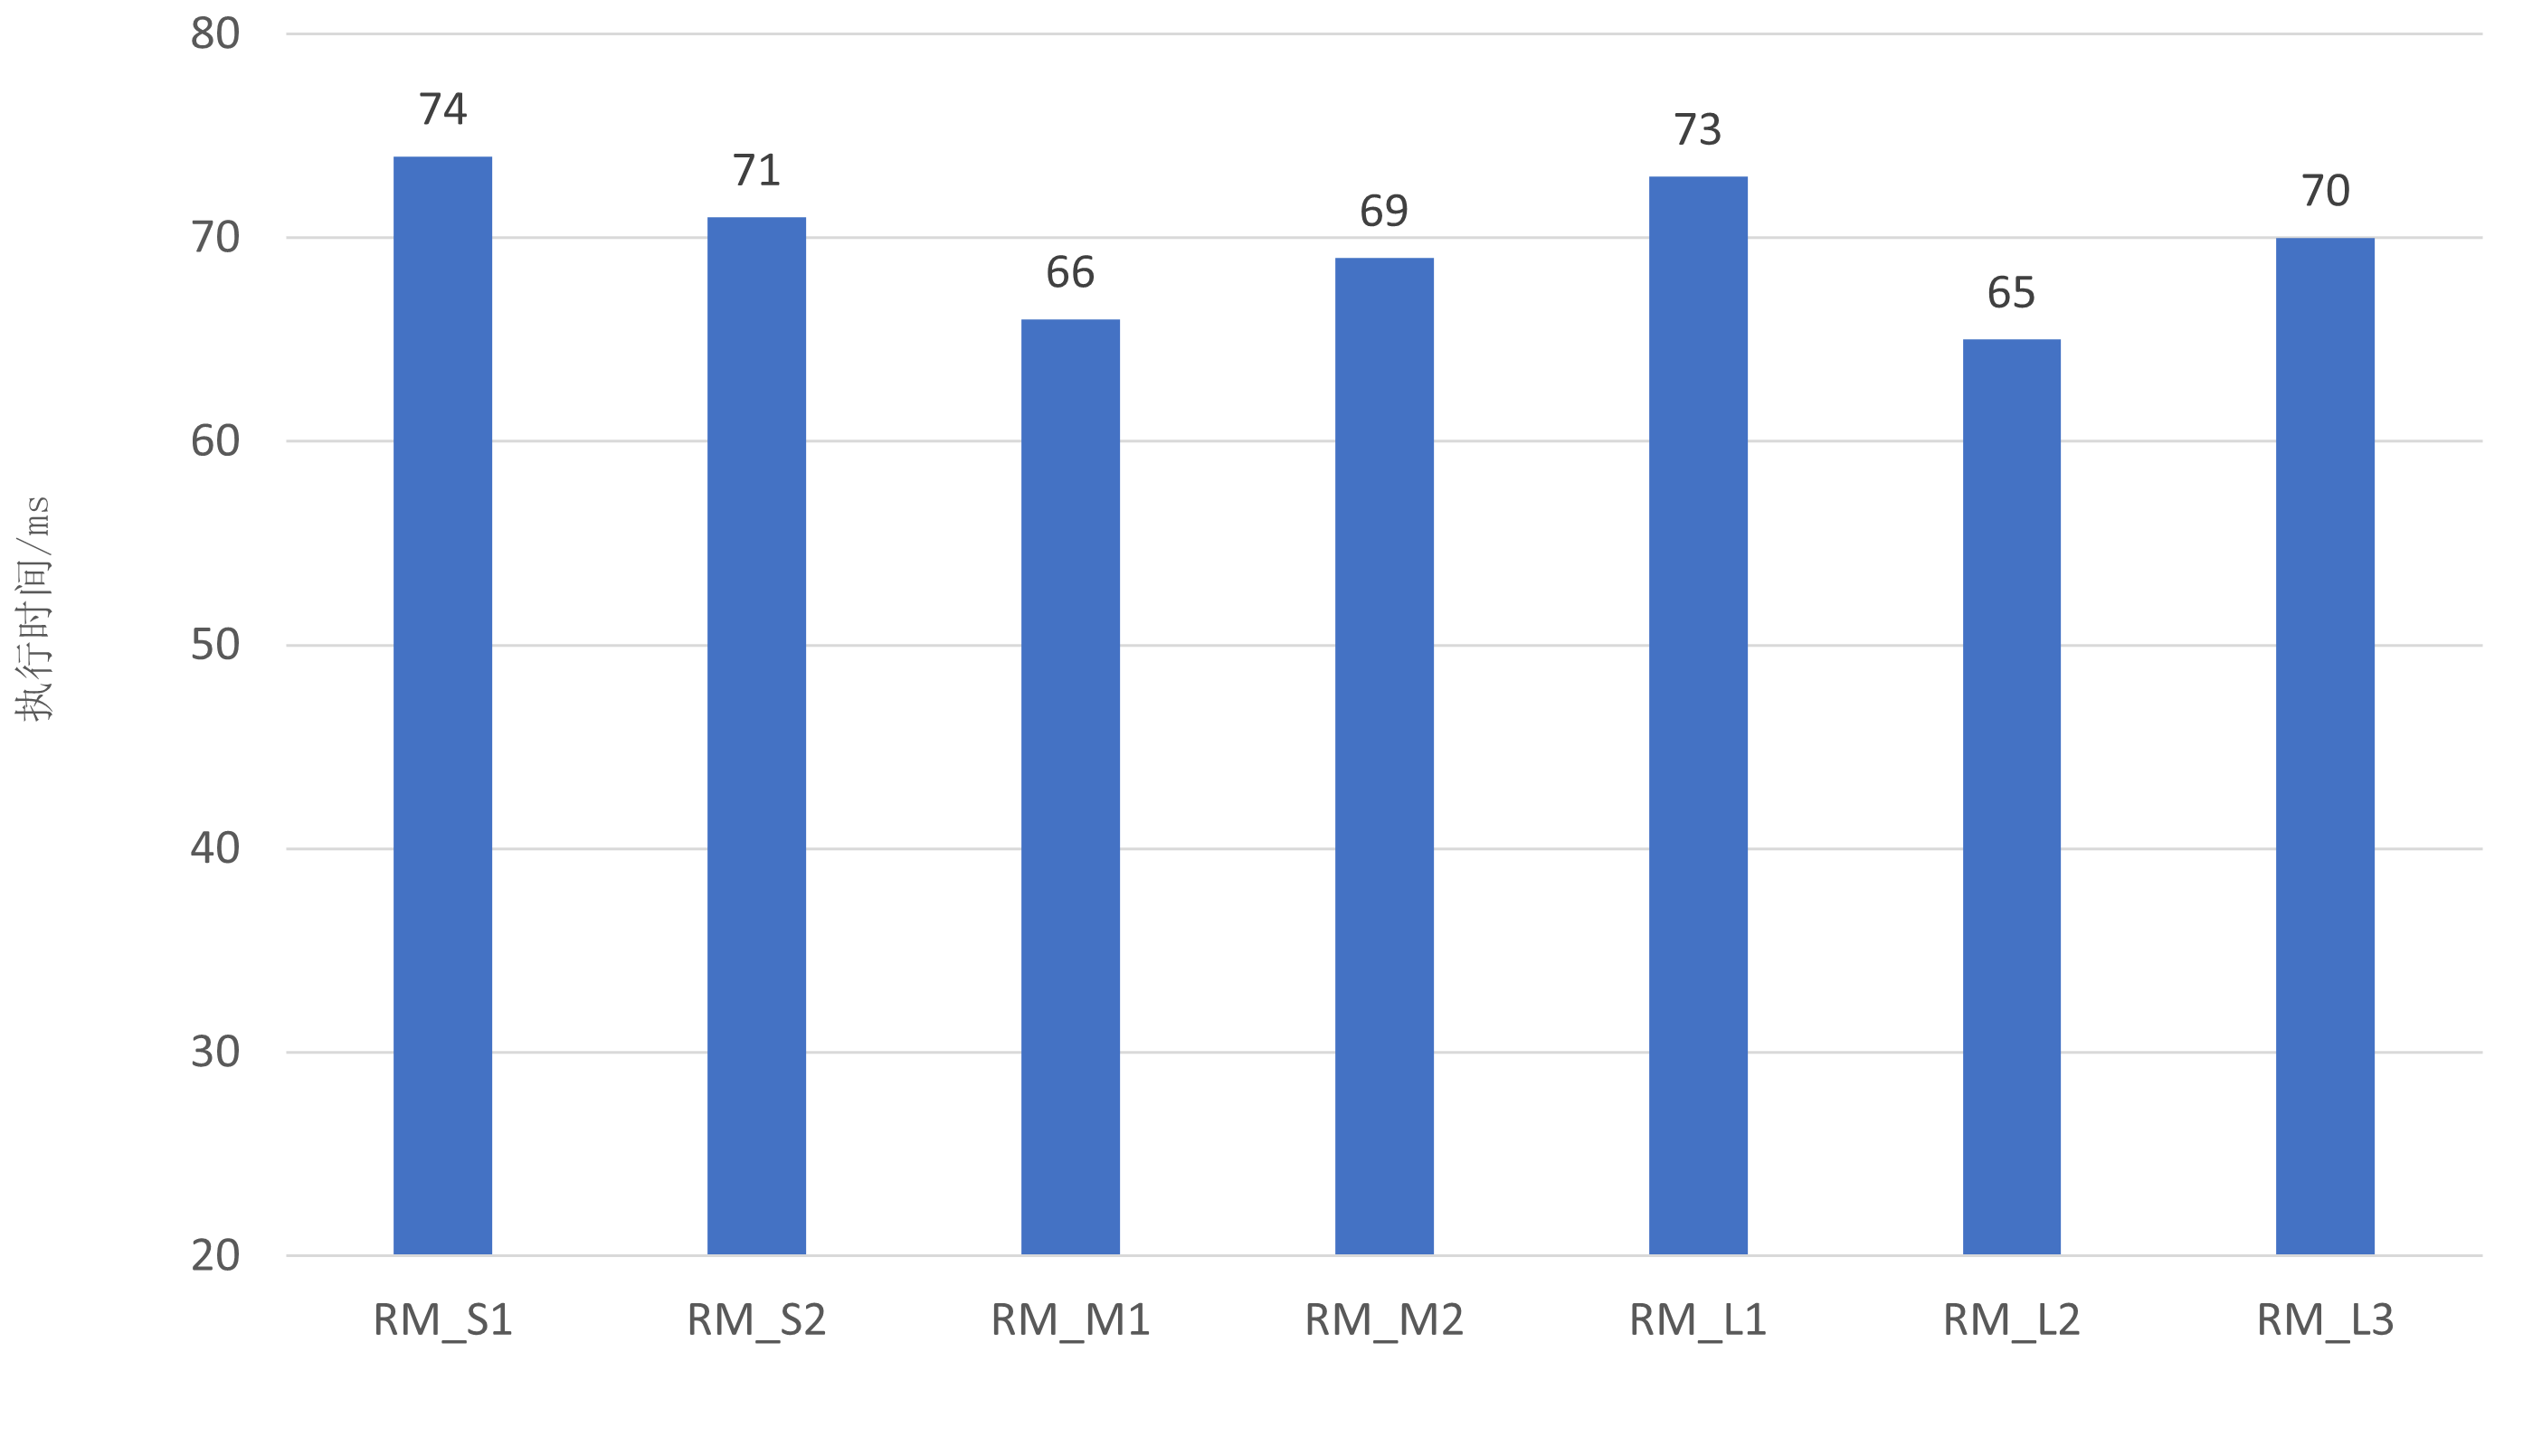
\includegraphics[width=0.8\textwidth]{e6.png}
  \caption{向量化策略算例性能}
 \end{figure}

 \subsection{计算模块峰值性能}
 对于RM不稳定性过程模拟,其以电子力场为基础,本质是通过牛顿第二定律求解包括粒子坐标,速度,受力矢量等物理量的过程。在不引入复杂状态方程与额外通信负载的条件下,电子势函数模拟实质是一类计算密集型应用。为了对比不同优化措施对计算模块的直接作用与收益,本节设计了针对计算单元的性能评估与分析,包括$Li/H_2$电子力场模拟在读写不同粒子规模与运行参数的场景,I/O与通信负载对计算在整个模拟流程的影响差异,这里在统计计算性能占比后,评估并分析并行模式与优化策略下计算单元的性能提升。

本节以$Li/H_2$电子力场模拟作为测试模型,运行环境为300核组,时间步选取为0.005fs,系综为NVE。图5.7展示了模拟流程中不同计算模块在总计算负载上的占比情况,从图中可以看出电子力场的系统总能量计算作为主要的耗时单元,占据了接近70\%的计算负载,其中包括粒子间库仑力的计算,以播报形态的pauli作用排斥能修正,对于这部分物理计算,乘除法甚至开方运算占据了很大一部分比例。对于数据结构初始化与截断半径的判断部分(paireff::compute)有着16.6\%的计算占比,其他初始化模型,配置邻接表,统计粒子参数共占据14.7\%的计算。

 \begin{figure}[h]
  \centering
  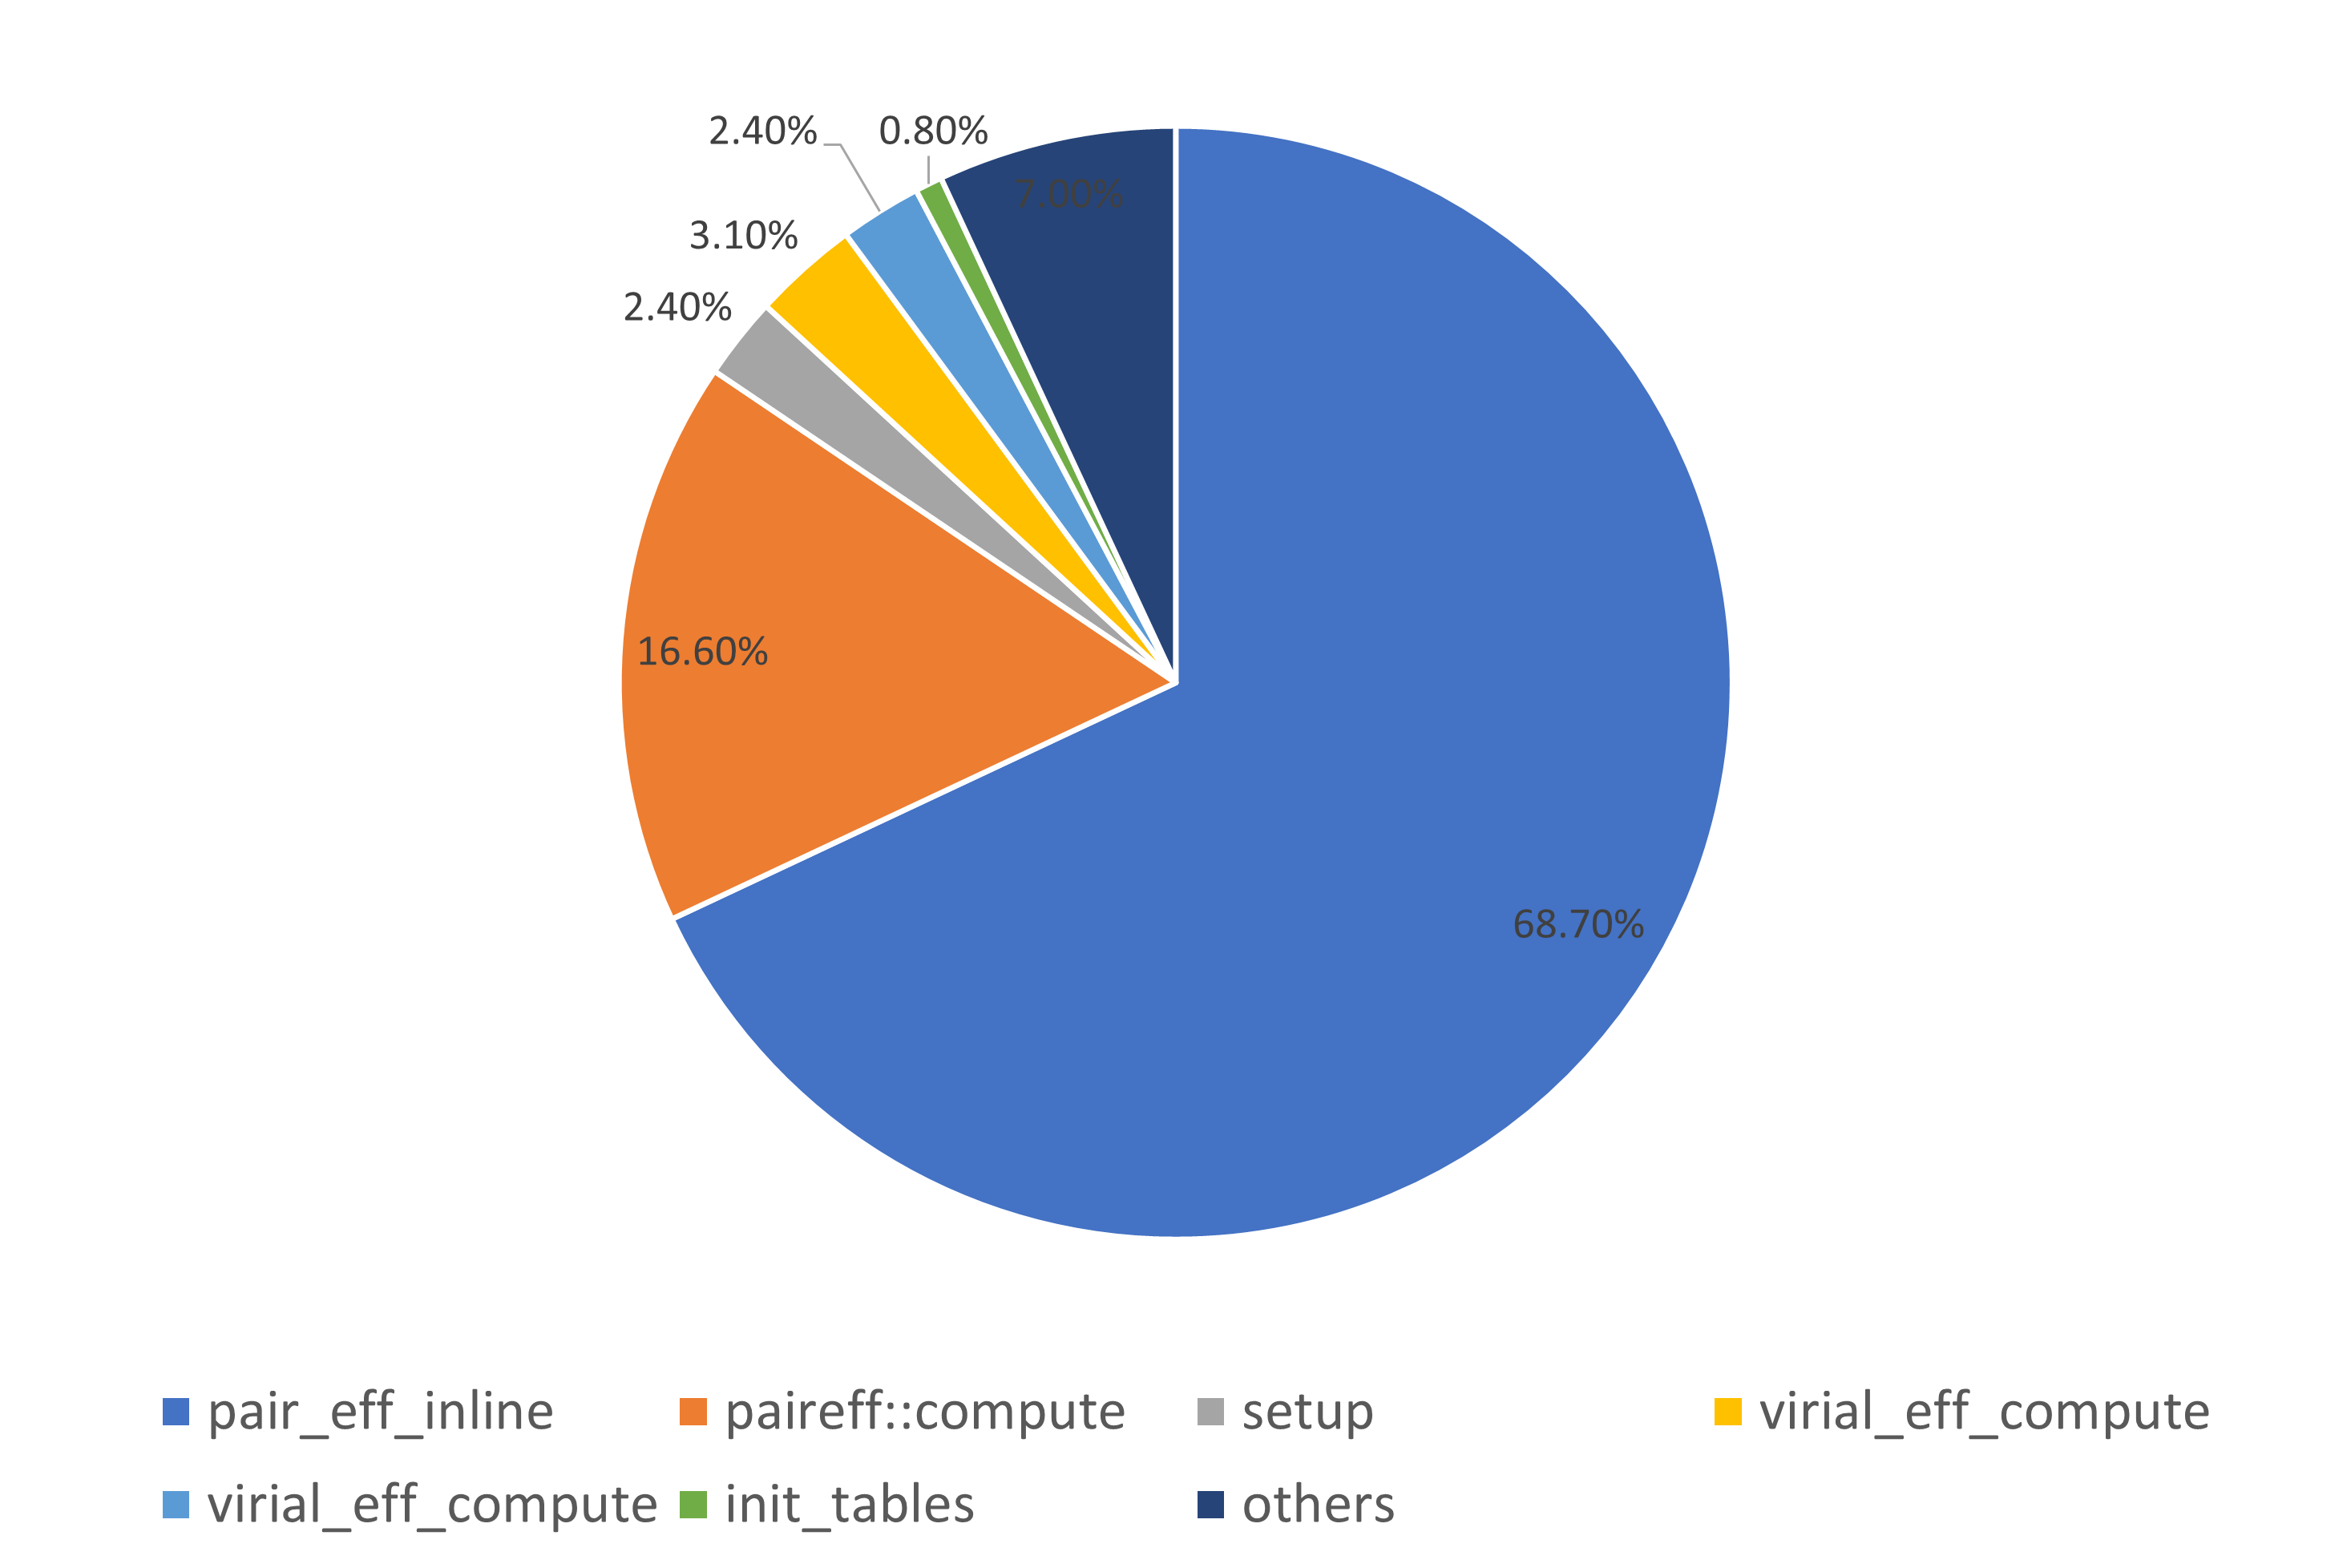
\includegraphics[width=0.8\textwidth]{cul5_1.png}
  \caption{计算模块负载占比}
 \end{figure}

 为了直观分析各计算模块的优化趋势与幅度,这里对重点占比模块进行分解,以便能够细粒度获取各单元在优化方案下的提升空间。同时以多用例对实验结果进行覆盖,减少模型的自误差,提升准确性。图5.8展示了LAMMPS在进行冲击激波诱导下的电子力场下,主要计算单元的优化加速比。所有计算单元的加速比落在了3.2x至7.2x区域内,造成不同计算单元性能差异的主要原因是各单元计算特征,以及计算密度受限。其中电子力场势函数的核心计算,即原子与成波包电子作用力的计算部分,主要是针对粒子矢量受力与动能的推导与修正,涵盖了大量的计算指令,而分支跳转与存储指令较少,使得并行优化策略高效覆盖,加速比在7x左右。而在势函数计算结构初始化,结果统计等非核心计算区域,加速比仅为3x到4x,一方面是进程在计算的同时存在相当比例的交叉通信,另一方面因为网格内粒子密度不同,频繁的数据交换也会影响计算性能的充分发挥。

  \begin{figure}[h]
  \centering
  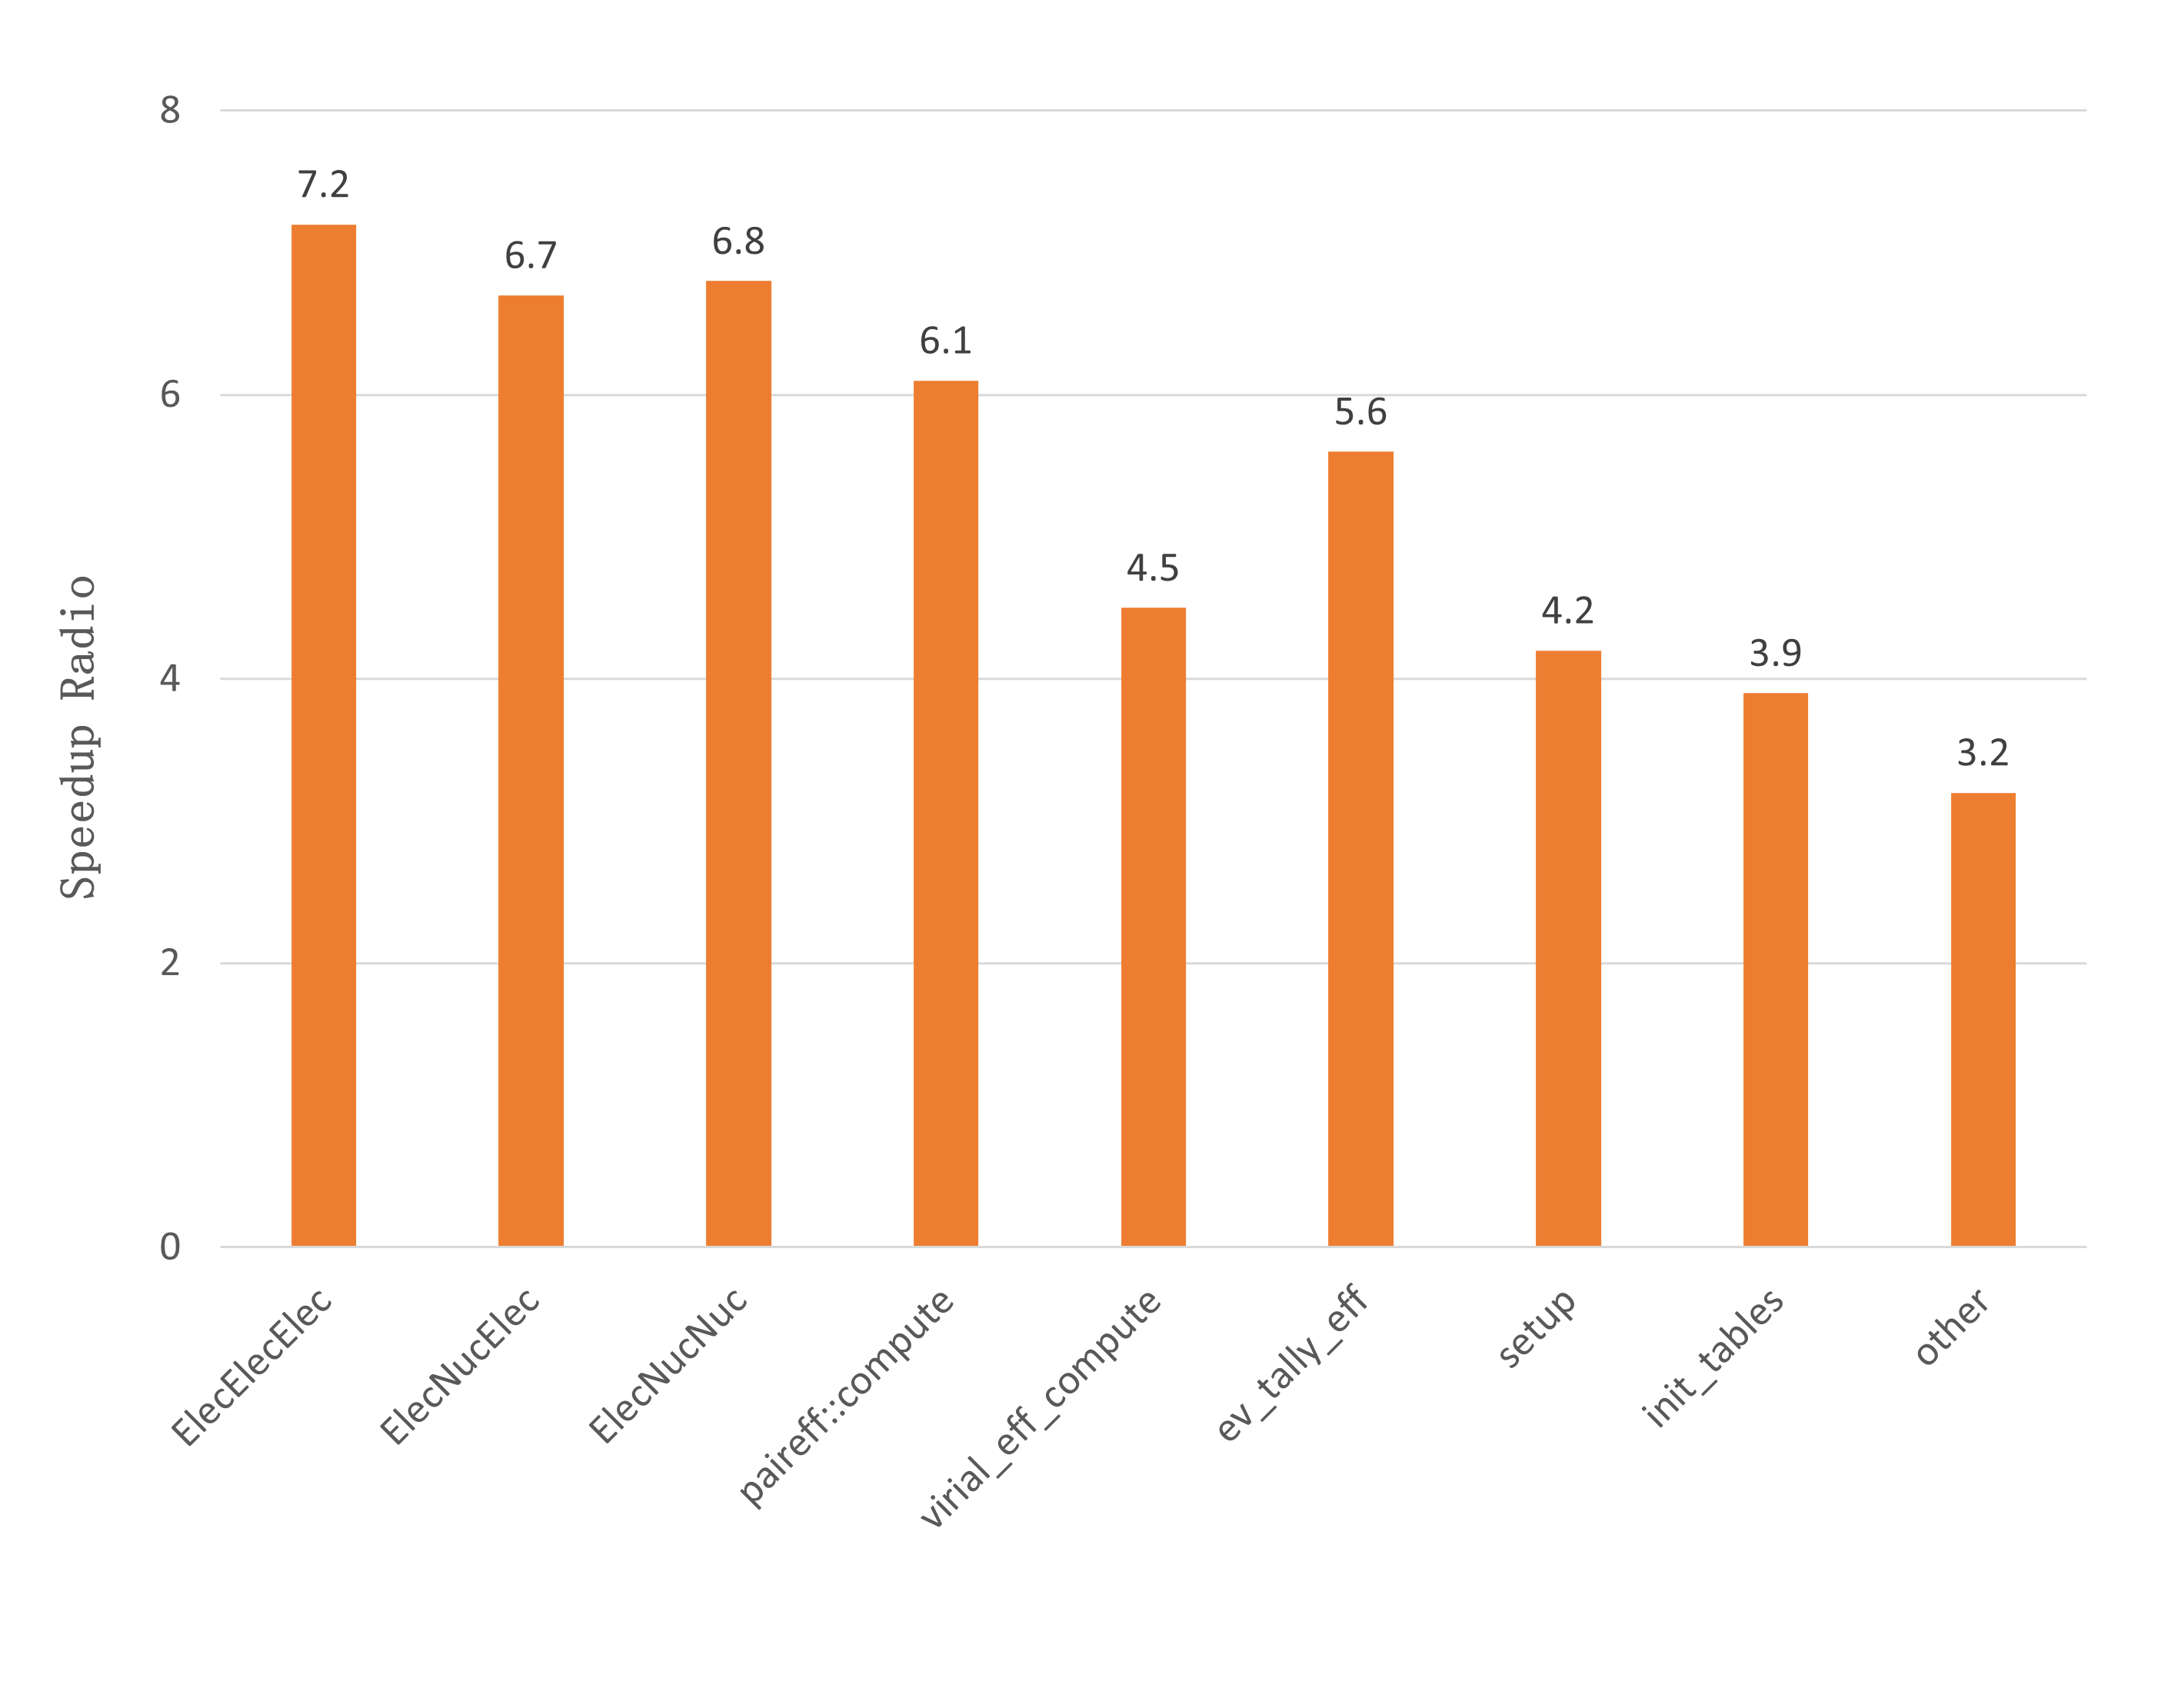
\includegraphics[width=0.8\textwidth]{cul5_2.png}
  \caption{计算模块性能提升}
 \end{figure}

\subsection{整体应用性能}
 通过性能测试的结果我们可以看出,在只通过主核进行计算时,每个时间步迭代的时间达到了 6794ms,这是由于主核在计算过程中不仅要完成热点函数的计算部分,还有进行I/O 操作,任务分发等工作,并且主核内的计算单元相对不足,导致性能结果不佳。在采用内层循环并行方案后,可以看到计算耗时有个明显地下降,这里是因为从核阵列的加入,使得邻居粒子的计算能够均匀分配到每个从核上,热点函数计算速度大幅提升,与此同时又引入了从核访存的开销问题。这里我们可以看出在使用 64 个从核同时进行计算后,整体的时间并没有表现出预取等比例地下降,因为仅仅引入计算的并行策略,增加访存开销的同时,也无法合理利用从核访存带宽。单次的 gld/gst 请求就会占用数百个时钟周期,此时访存开销成为了阻碍性能发挥的关键。在进行DMA 访存优化时,我们将原本需要多次访问才获取到的大块连续数据利用 DMA 方法采用单次的读写操作即可一次完成。这不仅降低了从核阵列内由于计算密度带来的频繁访存,也缓解了整体访存带宽的压力,至此的优化方法仅是对通用策略上的分析,还没有利用应用的具体特征进行深度优化。接下来通过更新并行策略来继续提高访存性能,采用单端更新的方法通过牺牲部分计算量,来换取更高的访存性能和并行度,这种方法支持大规模计算体系,扩展性也更强。尤其对于计算量较小,粒子排布较为稀疏的情况下发挥更好,从实验结果可以看出,针对 eFF 计算这种两体势来说,性能提升也较为明显,缺点就是固然会提升一定的计算量,但这种计算与访存性能之间的平衡却值得一试。为了进一步利用邻居粒子的局部性特征,通过在LDM 上开辟额外空间实现软件Cache 的做法也命中了超过百分之六十的粒子数据,访存频率和平均访存时间大幅减少,但软件Cache 实现的复杂性使其在性能提升方面不能与通用 CPU 上的多级 Cache 设计相比。至此,已经完成了对访存性能全部优化策略的分析。由于访存开销在整个体系计算中的比例降低和在单端更新并行方法中引入了更多的计算量,导致计算部分在势函数计算中占据了更大的部分。这里继续通过向量化指令和向量混洗操作,解决了离散粒子数据的读取和分支计算问题,使计算时间大幅降低。
 
 \begin{figure}[h]
  \centering
  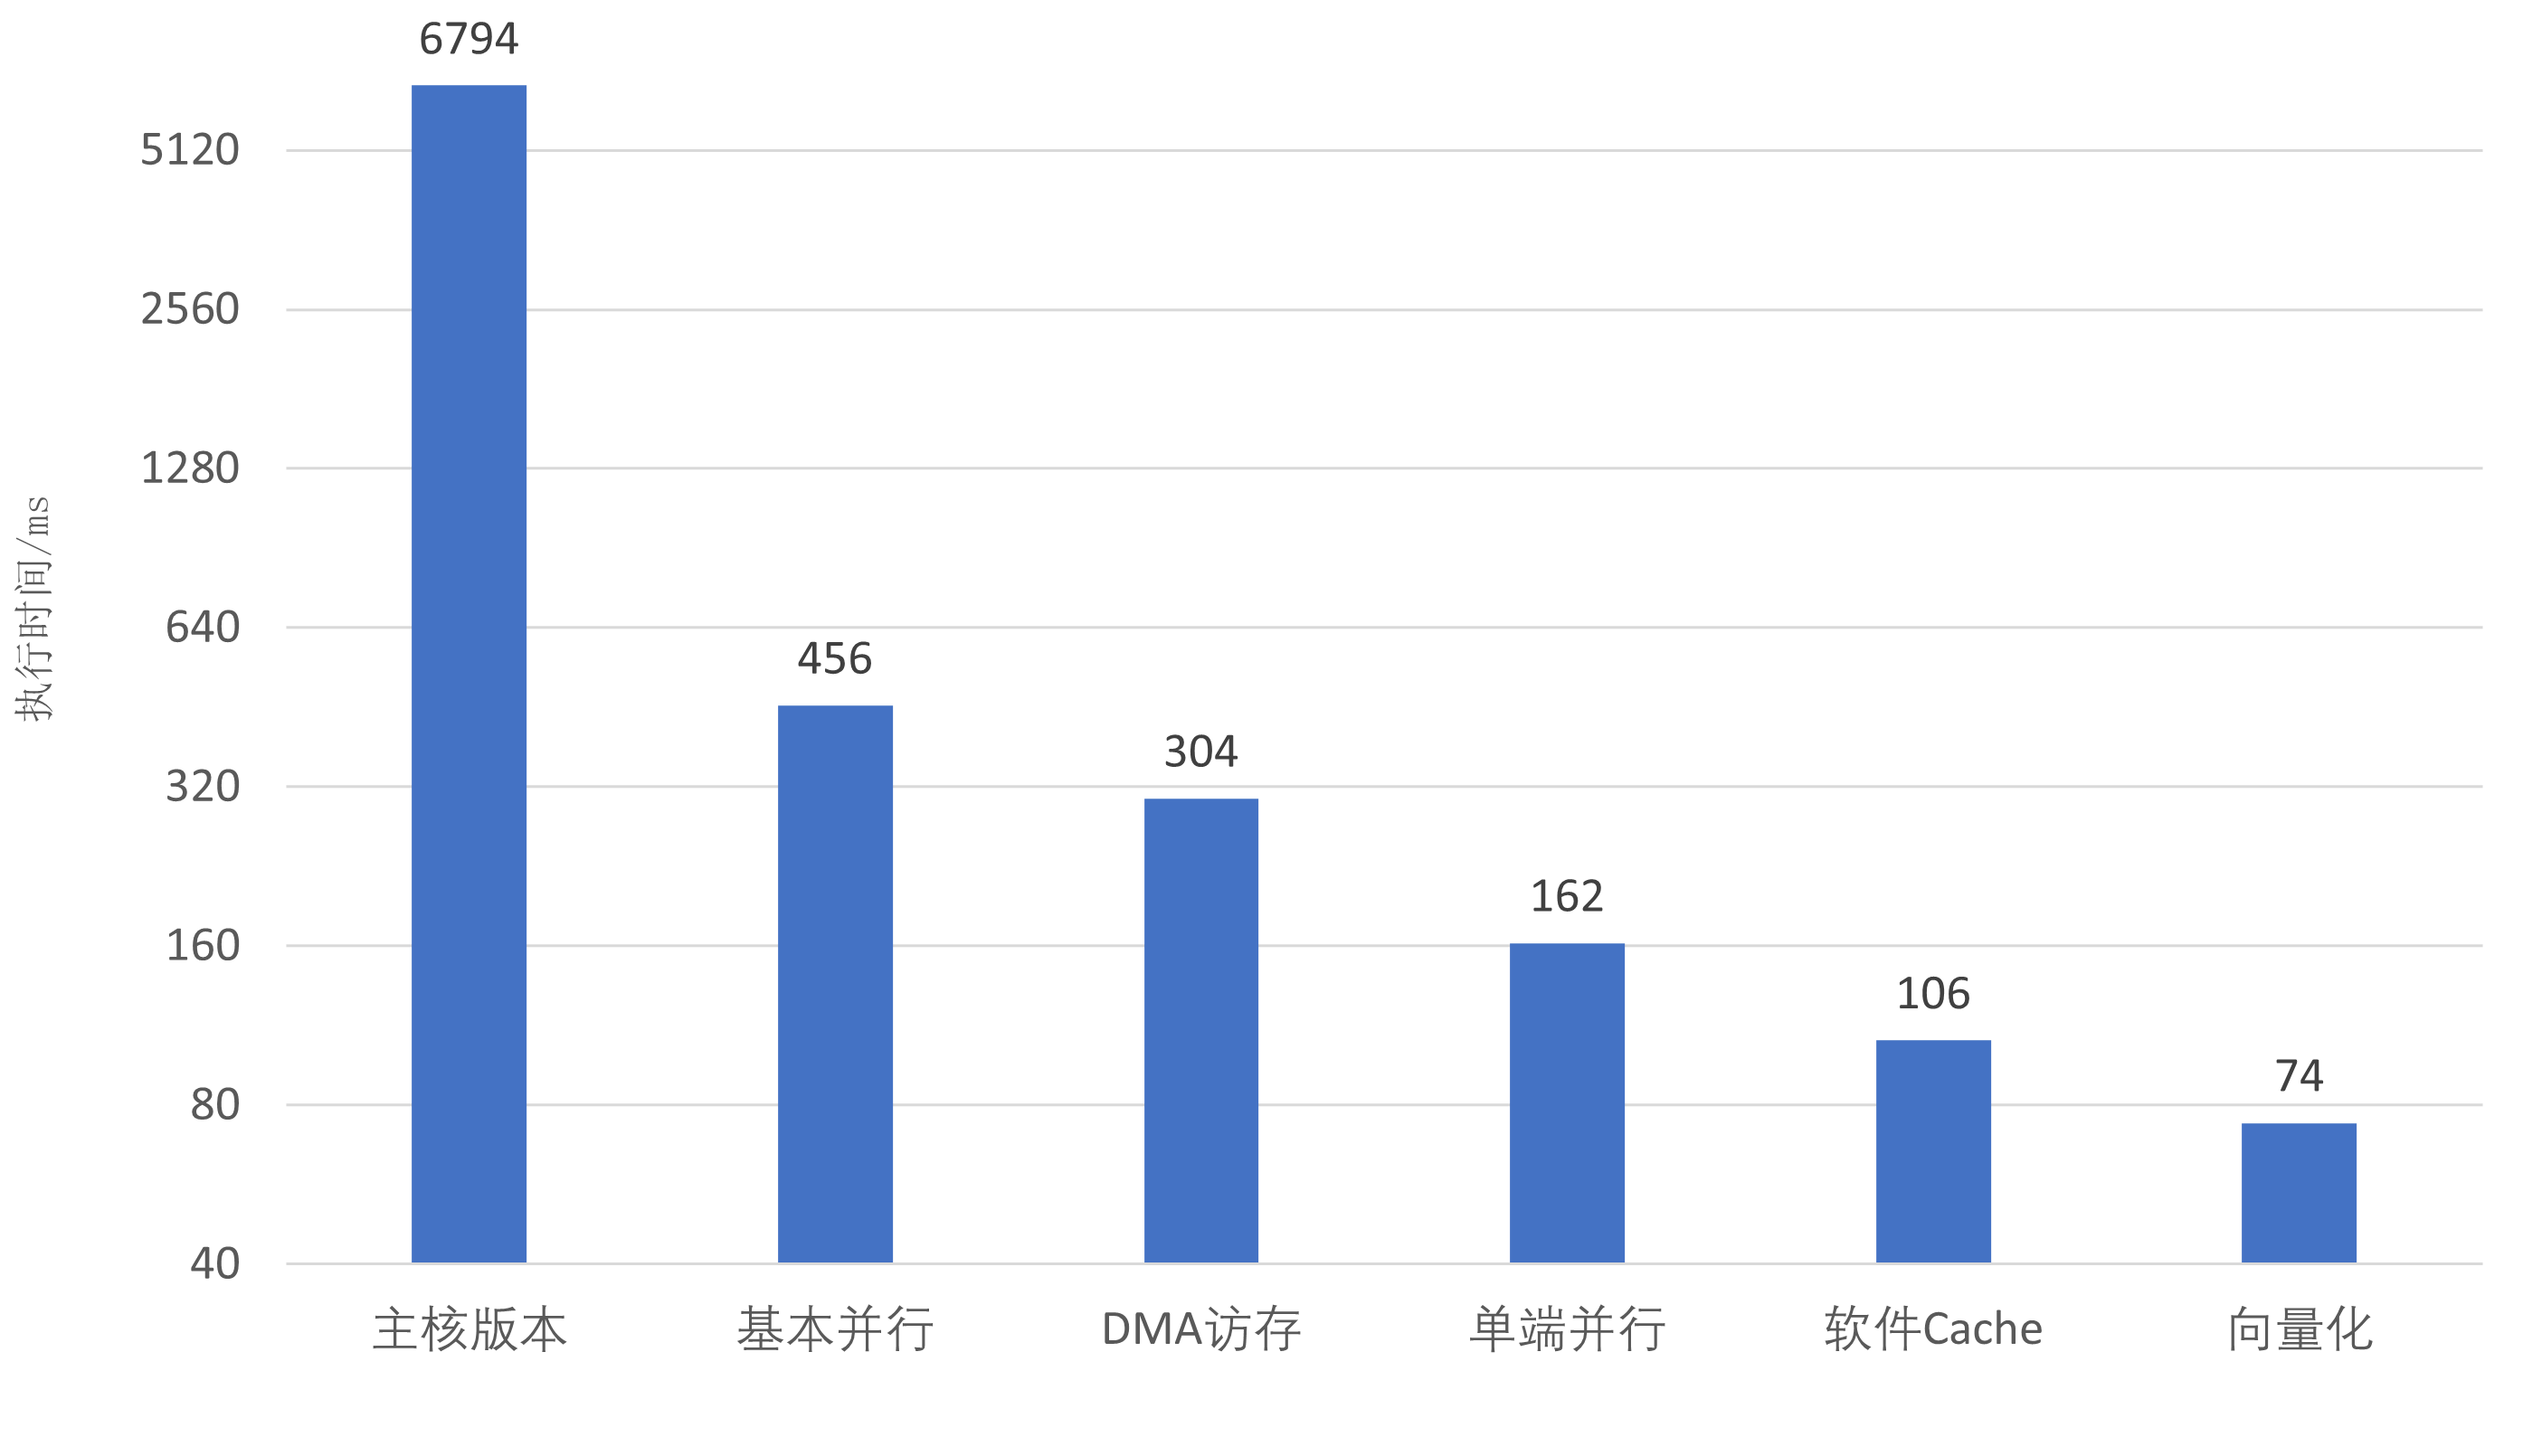
\includegraphics[width=0.8\textwidth]{opt_exp.png}
  \caption{不同优化配置下LAMMPS 的执行时间}
 \end{figure}
 
除了对不同实验配置和优化方案给出量化的性能结果外,这里也展示了在采用多个并行和优化方法的过程中,每种优化方案单独的性能提升在总性能优化中的地位,这同时也可以看出 eFF 势函数计算中对于不同应用特征每种策略产生的优化效果,也可以对访存,计算,通信等在申威平台上常见的处理问题进行总结。这里多种方案以不同的顺序进行累加测试后优化幅度可能会略有差异,例如采用单端更新方法会提升计算量,从而提高向量化的优化比例。

进行神威·太湖之光上各优化策略的性能测试后,这里也设计了不同优化阶段与通过 X86 平台上 eFF 势计算性能的对比实验。其中通用平台采用的计算核心数量与从核进行数量保持一致,采用相同的算例进行测试。可以看出通用处理器的性能与进行从核并行与访存优化后的性能相接近。这一方面是因为通用处理器的访存带宽要高于 SW26010 处理器,另一方面是多层 Cache 的设计使得数据重用性有着大幅的改善,访存频率也有着显著的降低。在从核采用软件Cache和向量化方法之后,访存和计算效率有了很大改善,性能也随之进行了反超。

 \begin{figure}[h]
  \centering
  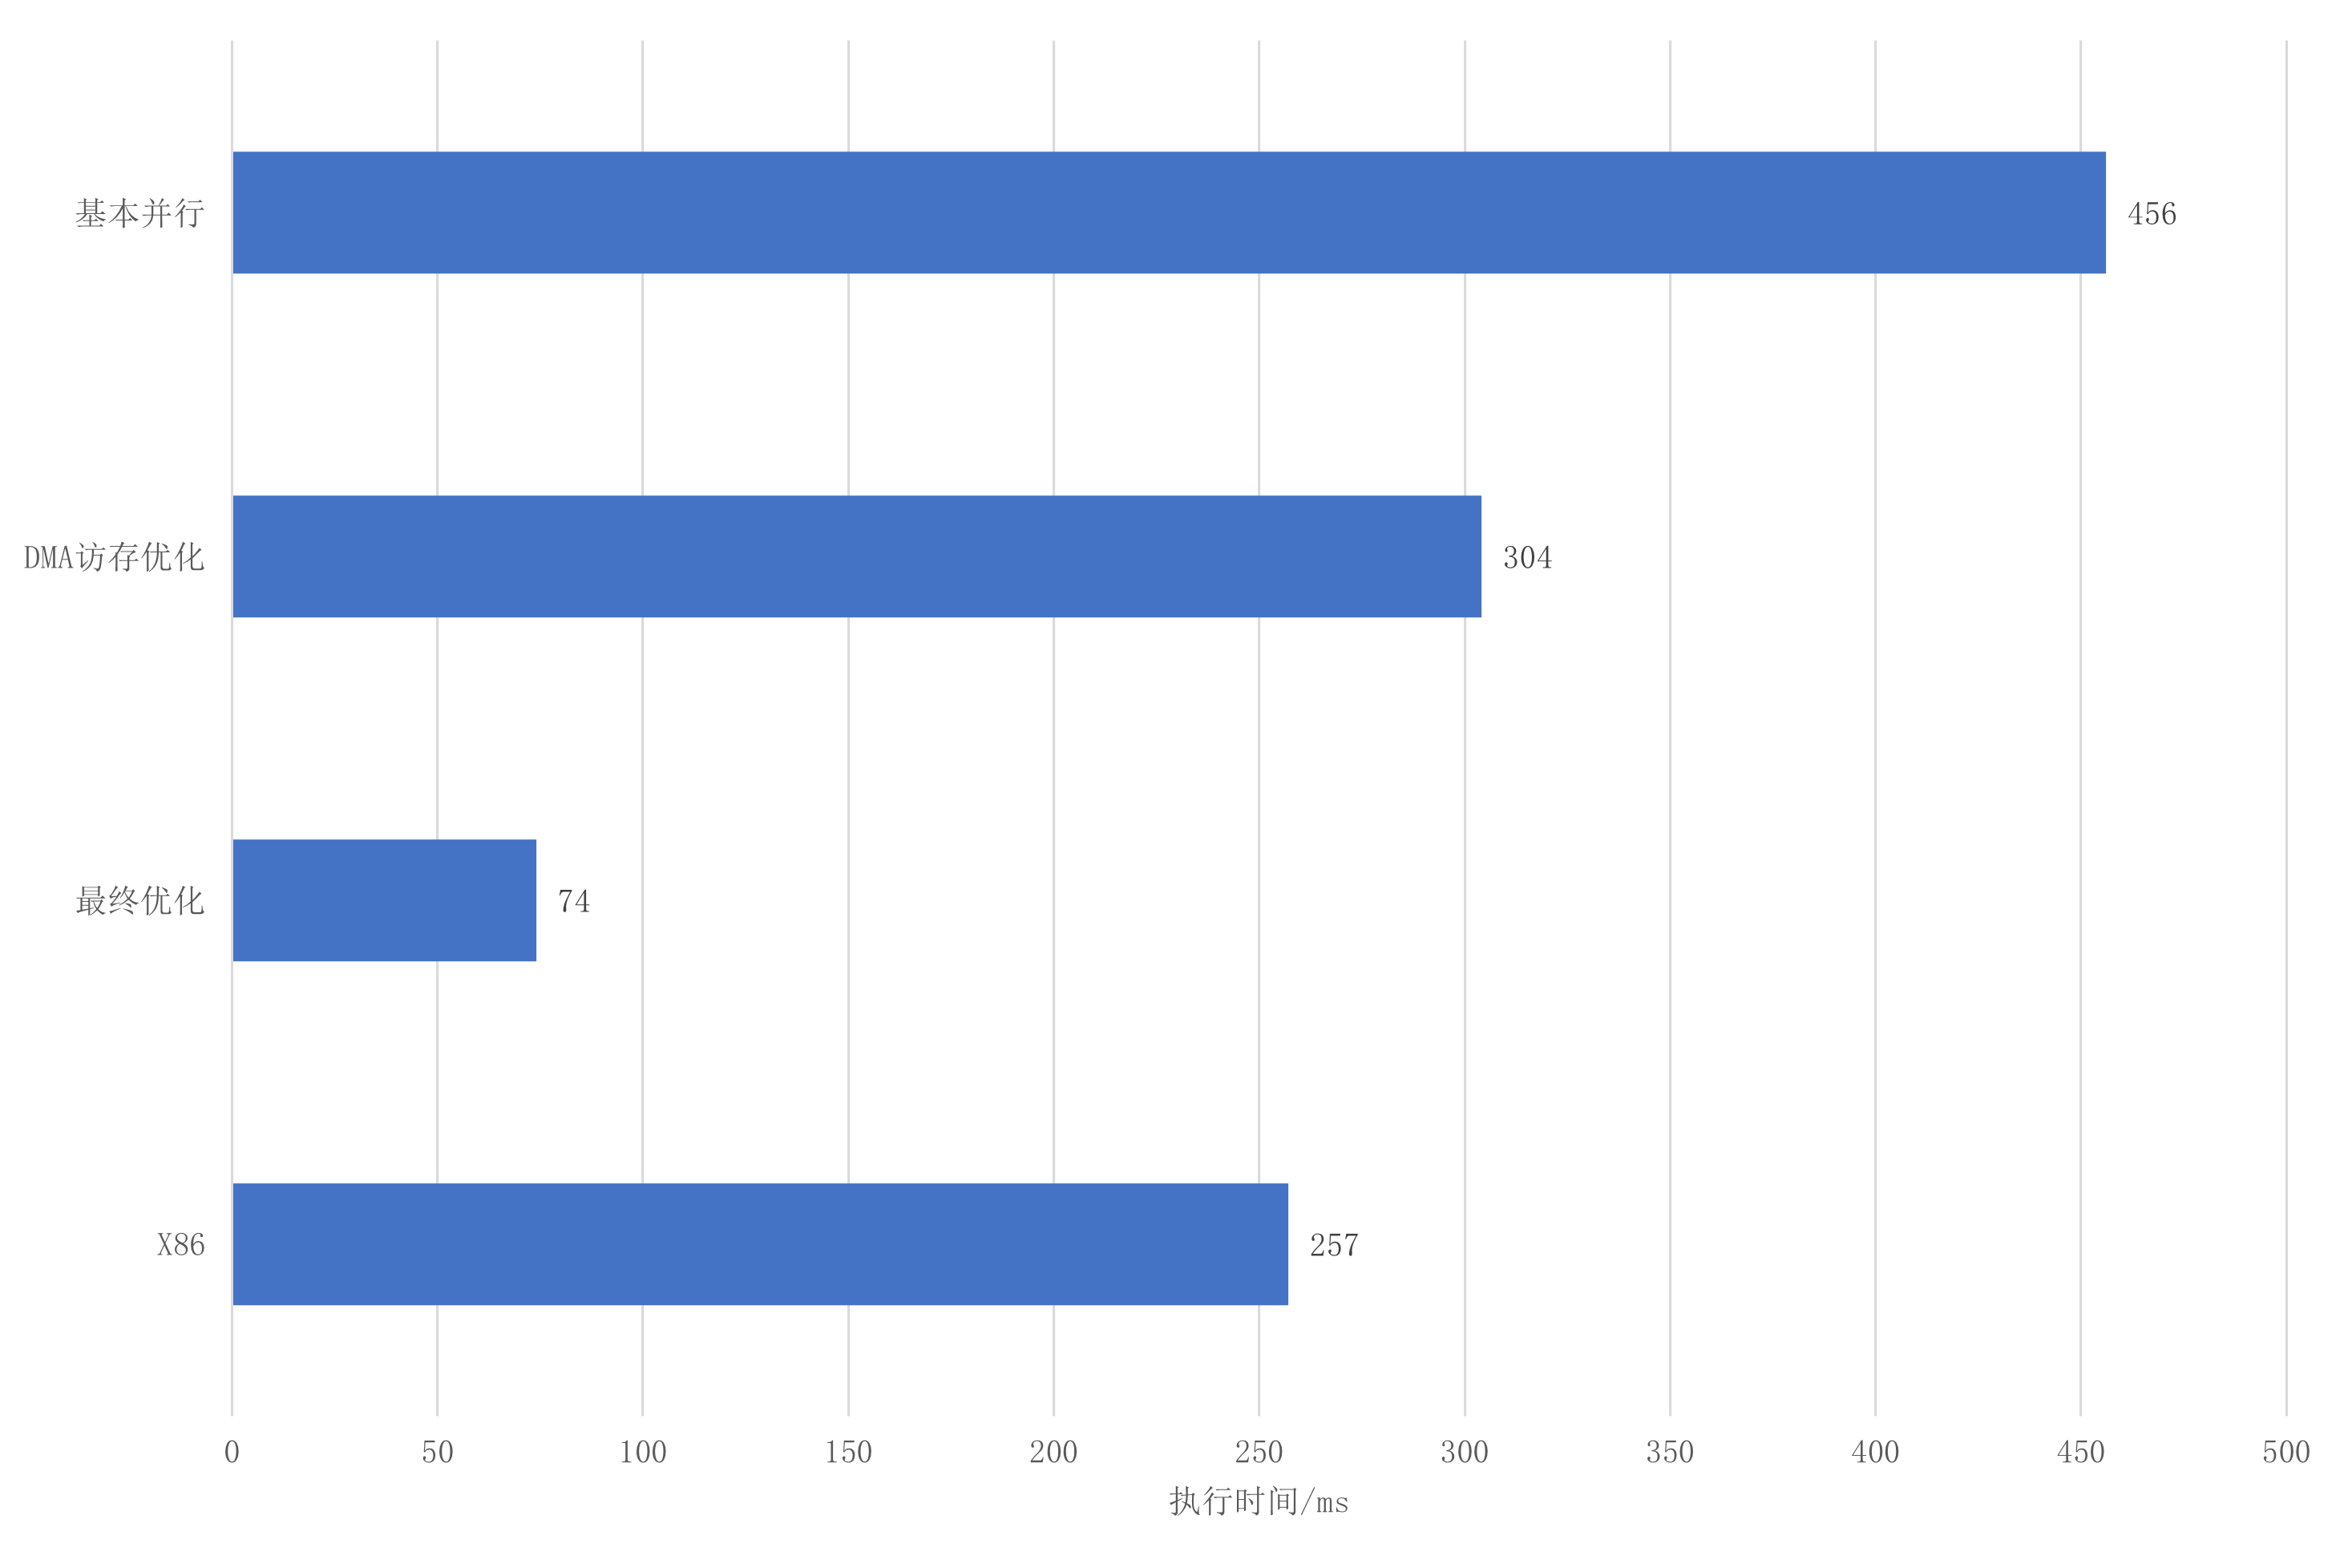
\includegraphics[width=0.8\textwidth]{platf_exp.png}
  \caption{申威平台LAMMPS 性能与通用平台比较}
\end{figure}

为了保证在程序算法在进行并行优化后,结果不会产生影响正确性的误差,这里还设计了程序正确性上的比对。通过比较在申威平台与通用平台上的计算结果,来保证结果的一致性,这里使用与上述相同的计算算例,选择了50000 个时间步作为模拟时长,在模拟过程中比较温度的变化来验证结果正确性。采用全部优化策略后的方案与通用平台上的计算温度的变化如图所示,从图中可以看出,在整个模拟进行的过程中,通用平台与优化后算法在相同算例下的温度变化基本一致。

\section{扩展性测试}
在分析完每一种优化方案对应用性能的提升幅度后,进行神威·太湖之光平台上 eFF 势函数计算的扩展性测试,进而总结出这部分计算在大规模模拟时的计算性能。这里的扩展性实验共分为两部分,强扩展性测试和弱扩展性测试,其中强扩展性时再总计算规模固定时,随着计算处理单元的递增,程序性能表现出来的趋势。弱扩展性是指在每个处理单元分配相同的任务量,随着计算规模和处理器数量等比例增长,性能表现出来的趋势。这里给出扩展效率的表达公式:

\begin{equation}
  U_N=\frac{T_a}{T_N}\cdot \frac{a}{N}
\end{equation}

其中𝑈𝑁 表示在处理核心数量在a 和N 时的程序扩展性,T 表示程序运行的耗时。

首先进行强扩展性测试,在这部分测试中,选取 980 万的粒子规模进行计算,进程数从 4 个开始逐步递增,最大计算进程数达到 65536 个。在此基础上,先通过设置理想情况下的性能扩展性,也就是性能性能随着进程数同比例增加,再与当前规模下的实际性能进行对比,得出扩展效率。从结果中可以观察到,随着计算进程的增多,LAMMPS 的实际性能与理想性能之间的偏差逐渐增大。这是因为总计算规模不变的情况下,参与计算的进程数量不断提高,导致每个进程负责的粒子计算不断变少,在进程数达到最大的时候,每个进程只分配了不到200 个粒子,此时在进程反而边界粒子占据了多数,使得扩展效率只有不到百分之六十。

 \begin{figure}[h]
  \centering
  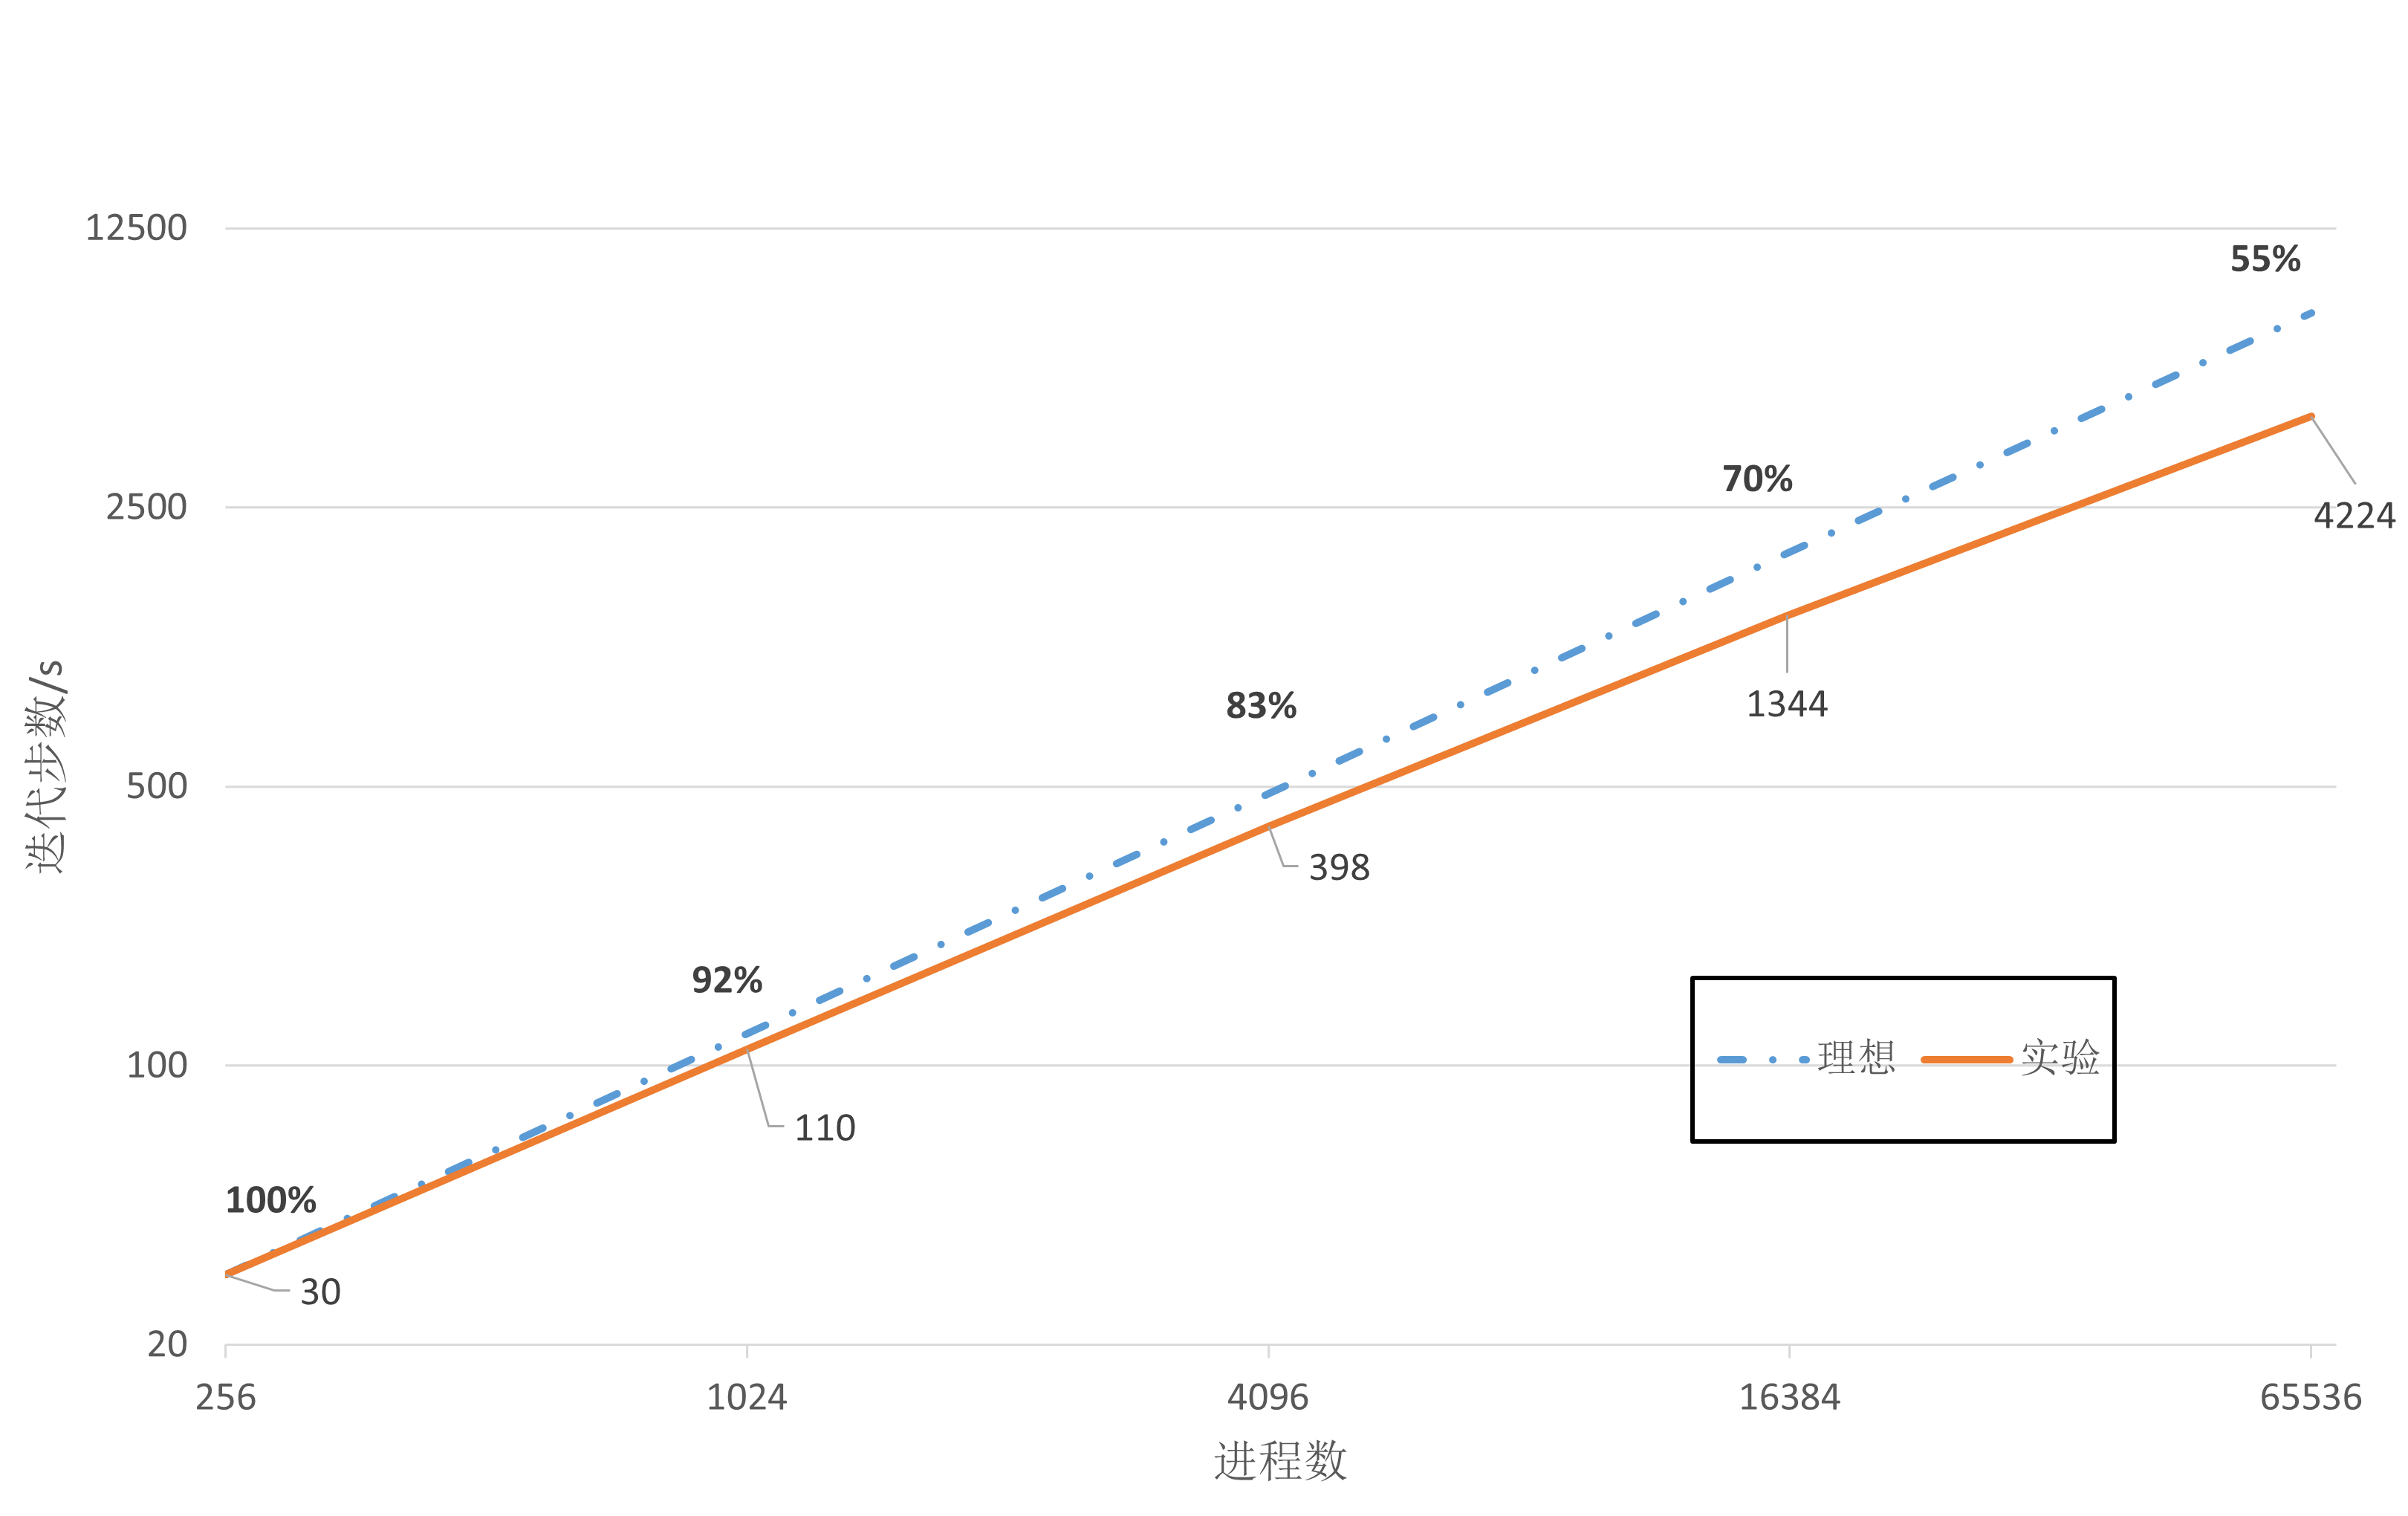
\includegraphics[width=0.8\textwidth]{s_scale.png}
  \caption{LAMMPS 强扩展性测试}
\end{figure}

 接下来进行弱扩展性测试,在这部分测试中,每个进程保持一定的粒子规模,算例总的粒子数随着进程数量等比例地增加,最大进程数同样达到65536 个。从结果中可以观察到,与强扩展性测试不同的是,整体扩展性不会随着进程数的增大而有着明显的变化,这是因为在每个进程中的粒子数量基本相同,进程在时间步之间的计算量不会发生太大的变化,所以弱扩展性的结果表现稳定的状态。

  \begin{figure}[h]
  \centering
  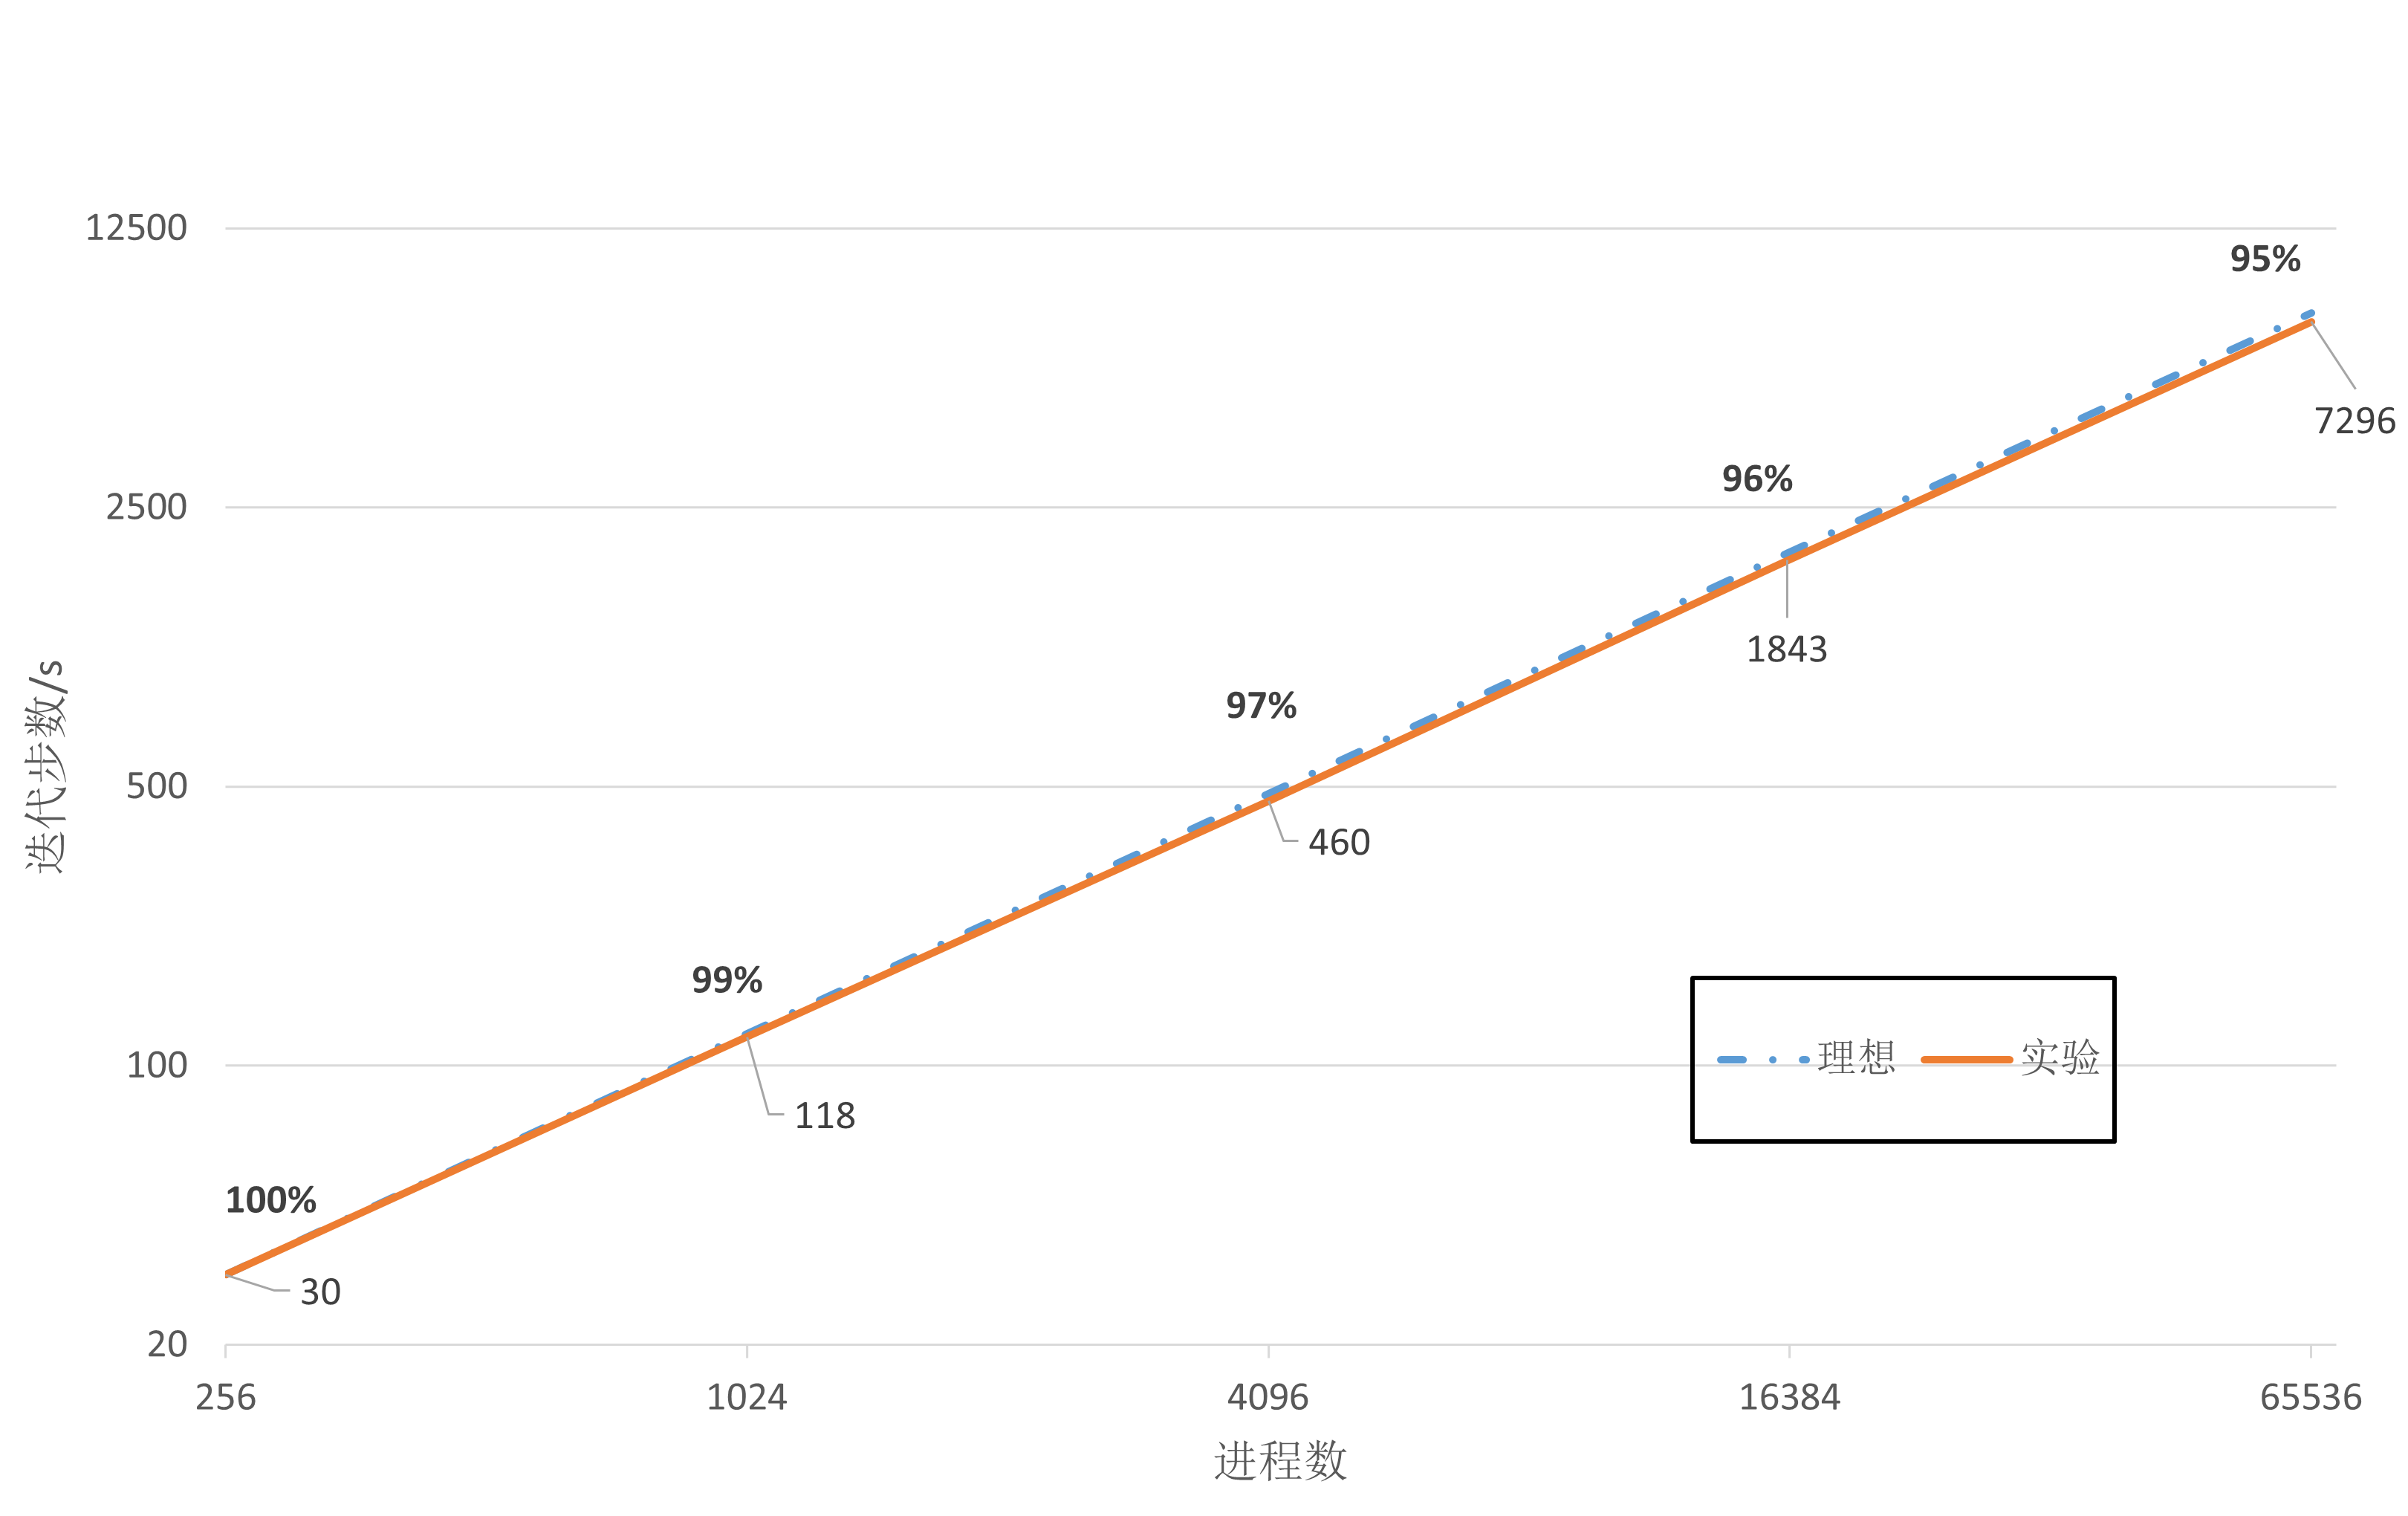
\includegraphics[width=0.8\textwidth]{w_scale.png}
  \caption{LAMMPS 弱扩展性测试}
\end{figure}

\section{本章小结}
本章展示出文章中提出优化策略的测试工作,涉及多种并行方案,访存,通信和计算的多种策略的性能分析,也给出了大规模计算中LAMMPS 的扩展性测试。首先测试了不同优化方案对于 eFF 势函数计算的性能提升情况,并通过方案间的具体加速比,分析了不同方案对总优化的贡献分配。测试表明在经过不同方案的性能加速后,并行版本的 eFF 计算相比于主核版本产生了 91 倍的性能提升,并且对于通用平台处理器,也有着不小的性能领先。在性能优化的同时验证了计算的正确性,使 X86 平台上的结果误差保持在可接受的范围内。接下来给出eFF 计算在神威·太湖之光上的扩展性测试,通过调整实际算例的规模,将计算进行增至 65536 个,分别得到了 55\% 的强扩展性和 88\% 的弱扩展性。
